\subsection{Gorenstein 环}

定义 1.--- 称环 A 为 Gorenstein 环，如果它是 Noether 的，并且 \(\mathrm{A}_{\mathfrak{m}}\) -模 \(\mathrm{A}_{\mathfrak{m}}\) 对 A 的每个极大理想 \(\mathfrak{m}\) 都具有有限内射维数。

为使 Noether 局部环 A 成为 Gorenstein 环，必须且只需 \(\mathrm{di}_{\mathrm{A}}(\mathrm{A})\) 有限；为使 Noether 环 A 成为 Gorenstein 环，必须且只需对 A 的每个极大理想 m，\(\Lambda_{m}\) 都如此。

命题 10.- 设 A 为 Gorenstein 环；则 A 是 Macaulay 环，且满足 \(\mathrm{di}_{\Lambda}(\mathrm{A}) = \dim(\mathrm{A})\) 。

对 A 的每个极大理想 m，有

\[
\begin{array}{l l} \dim (A _ {m}) & \leqslant \mathrm{di} _ {A _ {m}} (A _ {m}) \\ \mathrm{di} _ {A _ {m}} (A _ {m}) & = \operatorname{prof} (A _ {m}) \\ \operatorname{prof} (A _ {m}) & \leqslant \dim (A _ {m}) \end{array} \quad \begin{array}{l l} & (n ^ {\circ} 6, \text { prop. } 8) \\ & (n ^ {\circ} 6, \text { prop. } 9) \\ & (\S 1, n ^ {\circ} 4, \text { cor. } 2 \text { du   th. } 2); \end{array}
\]

由此推出 A 是 Macaulay 环，并且通过取上确界得到 \(\mathrm{di}_{\mathrm{A}}(\mathrm{A}) = \dim(\mathrm{A})\) (第 2 节, 命题 3)。

于是，使 \(\mathrm{di}_{\mathrm{A}}(\mathrm{A})\) 有限的那些 Noether 环 A 正是维数有限的 Gorenstein 环 (第 2 节, 命题 3)，而使 A-模 A 为内射模的那些 Noether 环正是 Artin Gorenstein 环。

例. 1) 对 Gorenstein 环 A 的每个乘性子集 S，分式环 \(S^{-1}A\) 都是 Gorenstein 环：事实上，设 q 为 \(S^{-1}A\) 的一个极大理想；它形如 \(S^{-1}p\)，其中 p 是 A 的一个与 S 不相交的素理想。设 m 为 A 的包含 p 的一个极大理想；则环 \(B = (S^{-1}A)_q\) 同构于 \(A_p\) (II, § 2, 第 5 节, 命题 11)，从而同构于 \(A_m\) 的一个分式环，因此满足 \(\text{di}_B(B) < +\infty\) (第 2 节, 命题 3 的推论 1)。

\begin{enumerate}
\def\labelenumi{\arabic{enumi})}
\setcounter{enumi}{1}
\item
  设 A 为 Gorenstein 环，J 为 A 的一个由 A-正则序列 x 生成的理想。商环 A/J 是 Gorenstein 环：事实上，对 A 的每个包含 J 的极大理想 m，序列 x 在 \(A_{m}\) 中的像是 \(A_{m}\) -正则的且生成理想 \(J_{m}\)，于是由第 4 节, 命题 7 的推论，\(A_{m}/J_{m}\) 是 Gorenstein 环。
\item
  设 A 为 Noether 局部环，J 为 A 的一个理想，它由 \(\mathfrak{m}_{\mathrm{A}}\) 中元素组成的 A-正则序列生成。若 A/J 是 Gorenstein 环，则 A 亦然 (第 4 节, 命题 7 的推论)。
\item
  设 A 为 Noether 正则局部环；则 A 是 Gorenstein 环。事实上，设 x 为 A 的一个坐标系 (VIII, § 5, 第 1 节, 定义 1)。序列 x 是 A-正则的（同上引文, 第 2 节, 定理 1）且生成理想 m\_A；因此可以应用例 3。
\item
  主理想环的每个商环都是 Gorenstein 环 (例 2)。特别地，域上的每个单生成代数都是 Gorenstein 环。
\end{enumerate}

引理 1.- 设 A 为 Artin 局部环。下列条件等价：

\begin{enumerate}
\def\labelenumi{(\roman{enumi})}
\item
  A 是 Gorenstein 环；
\item
  A-模 A 是内射的；
\item
  \(\kappa_{\mathrm{A}}\) -向量空间 \(\operatorname{Hom}_{\mathrm{A}}(\kappa_{\mathrm{A}}, \mathrm{A})\) 的维数为 1。
\end{enumerate}

回忆 (A, VIII, 第 3.5 页)：A 具有非零的极小理想；这样的理想是单模，从而同构于 \(\kappa_{\mathrm{A}}\) 。于是 \(\kappa_{\mathrm{A}}\) -向量空间 \(\mathrm{Hom}_{\mathrm{A}}(\kappa_{\mathrm{A}}, \Lambda)\) 非零；说它维数为 1，就是说 A 只含一个非零极小理想，它便是 A 的底座 (A, VIII, § 4, 第 6 节)。

(i) 与 (ii) 的等价性已在命题 10 之后证明。设 A-模 A 是内射的。设 \(x\) 与 \(y\) 为 A 的两个被 \(\mathfrak{m}_{\Lambda}\) 零化的非零元素。存在唯一的 A-线性映射 \(\varphi : Ax \to A\) 使 \(\varphi(x) = y\) ；由于 A 是内射的，它可扩张为 \(\Lambda\) 的一个自同态，这蕴含 \(y\) 属于 \(Ax\)，于是得到 (iii)。

反之，设 \(\mathrm{Hom}_{\mathrm{A}}(\kappa_{\mathrm{A}},\Lambda)\) 的维数为 1。设 M 为有限生成 A-模；它具有有限长度，从而具有一个合成列，其诸商都同构于 \(\kappa_{\mathrm{A}}\) 。由此对 M 的长度用归纳法，得到不等式 \(\mathrm{long}_{\mathrm{A}}(\mathrm{Hom}_{\mathrm{A}}(\mathrm{M},\Lambda)) \leqslant \mathrm{long}_{\mathrm{A}}(\mathrm{M})\) 。在扩张模的正合列

\[
0 \to \operatorname{Hom} _ {\mathrm{A}} (\kappa_ {\mathrm{A}}, \mathrm{A}) \longrightarrow \operatorname{Hom} _ {\mathrm{A}} (\mathrm{A}, \mathrm{A}) \stackrel {{\alpha}} {{\longrightarrow}} \operatorname{Hom} _ {\mathrm{A}} (\mathfrak {m} _ {\mathrm{A}}, \mathrm{A}) \longrightarrow \operatorname{Ext} _ {\mathrm{A}} ^ {1} (\kappa_ {\Lambda}, \mathrm{A}) \to 0,
\]

中因此有 \(\operatorname{long}_{\mathrm{A}}(\operatorname{Hom}_{\mathrm{A}}(\mathfrak{m}_{\mathrm{A}},\mathrm{A})) \leqslant \operatorname{long}_{\mathrm{A}}(\mathfrak{m}_{\mathrm{A}}) = \operatorname{long}(\mathrm{A}) - 1 = \operatorname{long}_{\mathrm{A}}(\operatorname{Im}\alpha)\) 。于是 \(\alpha\) 是满射，\(\operatorname{Ext}_{\mathrm{A}}^{1}(\kappa_{\mathrm{A}},\mathrm{A})\) 为零，且 A-模 A 是内射的 (第 3 节, 命题 4)。

引理 2.--- 设 \(\Lambda\) 为满足 \(\mathrm{di}_{\mathbf{A}}(\mathbf{A}) = +\infty\) 的 Noether 局部环。有 \(\operatorname{Ext}_{\mathbf{A}}^{i}(\kappa_{\Lambda}, \mathbf{A}) \neq 0\)（对每个整数 \(i \geqslant \dim(\mathbf{A})\)）。

对 \(\dim(A)\) 用归纳法。当 \(\dim(A) = 0\) 时，\(\mathfrak{m}_A\) 是 \(A\) 的唯一素理想，断言由第 3 节的命题 6 得出。于是设 \(\dim(A) > 0\)，并设 \(\mathfrak{p}\) 为 \(A\) 的一个异于 \(\mathfrak{m}_A\) 的素理想；这时有 \(\dim(A_{\mathfrak{p}}) < \dim(A)\)。若 \(\mathrm{di}_{A_{\mathfrak{p}}}(A_{\mathfrak{p}}) = +\infty\)，则归纳假设蕴含 \(\operatorname{Ext}_{A_{\mathfrak{p}}}^{j}(\kappa(\mathfrak{p}), A_{\mathfrak{p}}) \neq 0\)（对每个整数 \(j \geqslant \dim(A_{\mathfrak{p}})\)）；由 § 1, 第 7 节的引理 3，这蕴含 \(\operatorname{Ext}_{A}^{i}(\kappa_{A}, A) \neq 0\)（对每个整数 \(i \geqslant \dim(A_{\mathfrak{p}}) + \dim(A/\mathfrak{p})\)，特别地对 \(i \geqslant \dim(A)\)）(VIII, § 1, 第 3 节, 命题 8, b))。

尚需处理下列情形：\(\mathrm{di}_{\mathrm{A}}(\mathrm{A})\) 无限，但 \(A_{p}\) 的内射维数对 A 的每个异于 \(m_{A}\) 的素理想 p 都有限。对这样的理想，此时由命题 10 有 \(\mathrm{di}_{\mathrm{A}_{\mathfrak{p}}}(\mathrm{A}_{\mathfrak{p}})=\dim(\mathrm{A}_{\mathfrak{p}})<\dim(\mathrm{A})\)，从而 \(\operatorname{Ext}_{\mathrm{A}_{\mathfrak{p}}}^{i}(\kappa(\mathfrak{p}),\mathrm{A}_{\mathfrak{p}})=0\)（对 \(i\geqslant\dim(\Lambda)\)）。既然 \(\mathrm{di}_{\mathrm{A}}(\mathrm{A})\) 无限，第 3 节的命题 6 便迫使 \(\operatorname{Ext}_{\mathrm{A}}^{i}(\kappa_{\mathrm{A}},\mathrm{A})\neq0\)（对每个整数 \(i\geqslant\dim(\mathrm{A})\)）。

定理 2 (Bass). 设 A 为 Noether 局部环；令 \(d = \dim(A)\)。设 \(\mathbf{x} = \cdot(x_1, \ldots, x_d)\) 为由 \(\mathfrak{m}_A\) 中元素组成的一个极大割序列，并用 \(x\) 表示它生成的理想。下列条件等价：

\begin{enumerate}
\def\labelenumi{(\roman{enumi})}
\item
  A 是 Gorenstein 环；
\item
  有 \(\mathrm{di}_{\mathrm{A}}(\mathrm{A}) = d\)；
\item
  存在整数 \(i>d\) 使 \(\operatorname{Ext}_{\mathrm{A}}^{i}(\kappa_{\mathrm{A}},\mathrm{A})=0\)；
\item
  \(\operatorname{Ext}_{\mathrm{A}}^{i}(\kappa_{\mathrm{A}},\mathrm{A}) = 0\)（对 \(i < d\)），且 \(\kappa_{\mathrm{A}}\) -向量空间 \(\operatorname{Ext}_{\mathrm{A}}^{d}(\kappa_{\mathrm{A}},\mathrm{A})\) 的维数为 1；
\item
  环 A 是 Macaulay 的，且 \(\kappa_{\mathrm{A}}\) -向量空间 \(\operatorname{Hom}_{\Lambda}(\kappa_{\mathrm{A}}, \mathrm{A}/x)\) 的维数为 1；
\item
  序列 \(\mathbf{x}\) 是 A-正则的，且 \(\kappa_{\mathrm{A}}\) -向量空间 \(\operatorname{Hom}_{\mathrm{A}}(\kappa_{\mathrm{A}},\mathrm{A} / x)\) 的维数为 1。
\end{enumerate}

(i)、(ii) 与 (iii) 的等价性由引理 2 及命题 10 得出。若 \(\mathrm{Ext}_{\mathrm{A}}^{i}(\kappa_{\mathrm{A}},\mathrm{A})\) 对每个整数 \(i < d\) 为零，则环 A 是 Macaulay 的 (§ 2, 第 3 节, 命题 3)；若环 A 是 Macaulay 的，则序列 x 是 A-正则的（同上引文, 定理 1）；若序列 x 是 A-正则的，则有 \(\mathrm{Ext}_{\mathrm{A}}^{i}(\kappa_{\mathrm{A}},\mathrm{A}) = 0\)（对 \(i < d\)），且 \(\kappa_{\mathrm{A}}\) -向量空间 \(\mathrm{Ext}_{\mathrm{A}}^{d}(\kappa_{\mathrm{A}},\mathrm{A})\) 与 \(\mathrm{Hom}_{\mathrm{A}}(\kappa_{\mathrm{A}},\mathrm{A}/x)\) 同构 (A, X, 第 166 页, 命题 9)。这就证明了条件 (iv)、(v) 与 (vi) 的等价性。

我们来证明 (i) 蕴含 (v)：若 A 是 Gorenstein 环，则它是 Macaulay 环 (命题 10)。于是序列 x 是 A-正则的 (§ 2, 第 3 节, 命题 4)，从而 A/x 是 Artin Gorenstein 环 (例 2)，故 \(\kappa_{\mathrm{A}}\) -向量空间 \(\mathrm{Hom}_{\mathrm{A}}(\kappa_{\mathrm{A}}, \mathrm{A}/x)\) 的维数为 1。

最后，我们来证明 (vi) 蕴含 (i)：在假设 (vi) 下，环 A/x 是 Gorenstein 环 (引理 1)，从而 A 是 Gorenstein 环 (例 3)。

推论.--- 设 Λ 为维数为 d 的 Noether 局部环。Λ-模 \(\operatorname{Ext}_{\mathrm{A}}^{d}(\mathbf{k}_{\mathrm{A}},\Lambda)\) 非零。

若 \(\Lambda\) 是 Gorenstein 环，这由定理 2 得出；否则由引理 2 得出。

命题 11.--- 设 A 为 Noether 环。下列条件等价：

\begin{enumerate}
\def\labelenumi{(\roman{enumi})}
\item
  A 是 Gorenstein 环；
\item
  对 A 的每个素理想 \(\mathfrak{p}\)，\(\kappa(\mathfrak{p})\) -向量空间 \(\operatorname{Ext}_{\Lambda_{\mathfrak{p}}}^{i}(\kappa(\mathfrak{p}),\mathrm{A}_{\mathfrak{p}})\) 在 \(i \neq \operatorname{ht}(\mathfrak{p})\) 时为零，而在 \(i = \operatorname{ht}(\mathfrak{p})\) 时维数为 1。
\item
  对 A 的每个极大理想 \(\mathfrak{m}\)，存在整数 \(i > \mathrm{ht}(\mathfrak{m})\) 使 \(\operatorname{Ext}_{\Lambda_{\mathfrak{m}}}^{i}(\mathrm{A}/\mathfrak{m},\mathrm{A}_{\mathfrak{m}}) = 0\) 。
\end{enumerate}

(i)⇒(ii)：这由把定理 2 应用于 Gorenstein 局部环 A \(_{p}\) 得出 (例 1)。

(ii)⇒(iii)：这是平凡的。

(iii)⇒(i)：在假设 (iii) 下，对 A 的每个极大理想 m，A \(_{m}\) 都是 Gorenstein 环 (定理 2)，故 A 是 Gorenstein 的。

\subsection{Gorenstein 环与平坦代数}

命题 12. 设 \(\rho: A \to B\) 为 Noether 局部环之间的一个局部同态，它使 B 成为平坦 A-模。下列条件等价：

\begin{enumerate}
\def\labelenumi{(\roman{enumi})}
\item
  B 是 Gorenstein 环；
\item
  A 与 \(\kappa_{\Lambda} \otimes_{\Lambda} B\) 都是 Gorenstein 环。
\end{enumerate}

我们先处理环 A 与 B 都是 Artin 环的情形。用 C 表示局部环 \(\kappa_{\Lambda} \otimes_{\mathrm{A}} \mathrm{B}\)；其剩余域 \(\kappa_{\mathrm{C}}\) 等同于 \(\kappa_{\mathrm{B}}\)。由于 B 在 A 上平坦，B-模 \(\operatorname{Hom}_{\mathrm{B}}(\mathrm{C}, \mathrm{B})\) 同构于 \(\operatorname{Hom}_{\mathrm{A}}(\kappa_{\mathrm{A}}, \mathrm{A}) \otimes_{\mathrm{A}} \mathrm{B}\) (I, § 2, 第 10 节, 命题 11)，从而同构于 \(\operatorname{Hom}_{\mathrm{A}}(\kappa_{\mathrm{A}}, \mathrm{A}) \otimes_{\kappa_{\Lambda}} \mathrm{C}\)。由此得出一列同构：

\[
\begin{array}{c} \operatorname{Hom} _ {\mathrm{B}} (\kappa_ {\mathrm{B}}, \mathrm{B}) \longrightarrow \operatorname{Hom} _ {\mathrm{C}} (\kappa_ {\mathrm{C}}, \operatorname{Hom} _ {\mathrm{B}} (\mathrm{C}, \mathrm{B})) \dashrightarrow \operatorname{Hom} _ {\mathrm{C}} (\kappa_ {\mathrm{C}}, \operatorname{Hom} _ {\Lambda} (\kappa_ {\mathrm{A}}, \mathrm{A}) \otimes_ {\kappa_ {\mathrm{A}}} \mathrm{C}) \\ \longrightarrow \operatorname{Hom} _ {\Lambda} (\kappa_ {\Lambda}, \mathrm{A}) \otimes_ {\kappa_ {\mathrm{A}}} \operatorname{Hom} _ {\mathrm{C}} (\kappa_ {\mathrm{C}}, \mathrm{C}). \end{array}
\]

特别地，有 \(\left[\mathrm{Hom}_{\mathrm{B}}(\kappa_{\mathrm{B}},\mathrm{B}):\kappa_{\mathrm{B}}\right] = \left[\mathrm{Hom}_{\mathrm{A}}(\kappa_{\mathrm{A}},\mathrm{A}):\kappa_{\mathrm{A}}\right]\left[\mathrm{Hom}_{\mathrm{C}}(\kappa_{\mathrm{C}},\mathrm{C}):\kappa_{\mathrm{C}}\right]\)，于是命题由第 7 节的引理 1 得出。

转到一般情形。如果在命题陈述中把“Gorenstein”一词换为“Macaulay”，则本命题是 § 2, 第 7 节命题 10 的一个特殊情形。于是可设环 A、B 与 C = \(\kappa_{\mathrm{A}} \otimes_{\mathrm{A}} \mathrm{B}\) 都是 Macaulay 的。B-模 C 是 Macaulay 的 (§ 2, 第 1 节, 例 4)。令 \(r = \dim(\mathrm{A})\)，\(s = \dim(\mathrm{C})\)。存在一个 A-正则序列 ( \(x_1, \ldots, x_r\) )，其元素属于 \(\mathfrak{m}_{\mathrm{A}}\)，以及一个序列 ( \(y_1, \ldots, y_s\) )，其元素属于 \(\mathfrak{m}_{\mathrm{B}}\) 且对 B-模 C 正则 (§ 2, 第 3 节, 命题 3)；用 \(x\) 表示前者生成的 A 的理想，用 \(\mathfrak{y}\) 表示后者生成的 B 的理想。序列 ( \(y_1, \ldots, y_s, \rho(x_1), \ldots, \rho(x_r)\) ) 是 B-正则的 (§ 1, 第 6 节, 命题 11)，且 A-模 B/ \(\mathfrak{y}\) 是平坦的（同上引文, 命题 10）。由 A/ \(x\) 到 B/(xB + \(\mathfrak{y}\) ) 的、由 \(\rho\) 出发取商得到的同态因此使 B/(xB + \(\mathfrak{y}\) ) 成为平坦的 (A/x)-模，且环 \(\kappa_{\mathrm{A}/x} \otimes_{\mathrm{A}/x} \mathrm{B}/(xB + \mathfrak{y})\) 同构于 C/ \(\mathfrak{y}\) C。于是，考虑到第 7 节的例 3，命题由证明的第一部分得出。

推论 1. -- 设 \(\mathfrak{p}: A \to B\) 为使 B 成为平坦 A-模的 Noether 环同态。下列条件等价：

\begin{enumerate}
\def\labelenumi{(\roman{enumi})}
\item
  B 是 Gorenstein 环；
\item
  （相应地 (iii)）对 B 的每个素理想（相应地极大理想）\(\mathfrak{q}\)，环 \(\mathrm{A}_{\mathfrak{p}^{-1}(\mathfrak{q})}\) 与 \(\kappa (\mathfrak{p}^{-1}(\mathfrak{q}))\otimes_{\mathrm{A}}\mathrm{B}\) 都是 Gorenstein 的。
\end{enumerate}

此外，若 B 是忠实平坦的 \(\Lambda\) -模，则这些条件蕴含 A 是 Gorenstein 环。

设 q 为 B 的一个素理想；令 \(\mathfrak{p} = \rho^{-1}(\mathfrak{q})\) 。环 \(B_{q}\) 同构于 \(B_{p}\) 的一个分式环，在 \(A_{p}\) 上平坦。为使 \(B_{q}\) 是 Gorenstein 环，必须且只需环 \(A_{p}\) 与 \(\kappa(\mathfrak{p}) \otimes_{A_{\mathfrak{p}}} B_{\mathfrak{q}}\) 都是 Gorenstein 环 (命题 12)。

\((\mathrm{i}) \Rightarrow (\mathrm{ii})\)：设 \(\mathfrak{q}\) 为 B 的一个素理想，并令 \(\mathfrak{p} = \rho^{-1}(\mathfrak{q})\)。若 B 是 Gorenstein 环，则 \(B_{\mathfrak{q}}\) 亦然；于是由前所证，\(A_{\mathfrak{p}}\) 与 \(\kappa(\mathfrak{p}) \otimes_{A_{\mathfrak{p}}} B_{\mathfrak{q}}\) 都是 Gorenstein 的。由 § 2, 第 6 节的注，\(\kappa(\mathfrak{p}) \otimes_{\mathrm{A}} B\) 在每个素理想处的局部化这时都是 Gorenstein 环，这蕴含 \(\kappa(\mathfrak{p}) \otimes_{\mathrm{A}} B\) 是 Gorenstein 环，从而得到 (ii)。

\begin{enumerate}
\def\labelenumi{(\roman{enumi})}
\setcounter{enumi}{1}
\tightlist
\item
  \(\Rightarrow\) (iii)：这是显然的。
\end{enumerate}

(iii)⇒(i)：对 B 的每个极大理想 n，由证明的开头（取 q = n 应用）可知 \(B_{n}\) 是 Gorenstein 环，从而得到 (i)。

若 B 是忠实平坦 A-模，则映射 \(^{q}\mathfrak{p}:\operatorname{Spec}(B)\longrightarrow\operatorname{Spec}(\Lambda)\) 是满射 (II, § 2, 第 5 节, 命题 11 的推论 4)，由此得到最后一个断言。

推论 2. 设 A 为 Noether 环，J 为 A 的理想，Â 为 A 关于 J-进拓扑的分离完备化。考察下列条件：

\begin{enumerate}
\def\labelenumi{(\roman{enumi})}
\item
  A 是 Gorenstein 环；
\item
  \(\widehat{\mathrm{A}}\) 是 Gorenstein 环；
\item
  对 A 的每个包含 J 的极大理想 m，\(A_{m}\) 是 Gorenstein 环；
\item
  对 A 的每个满足 \(p + J \neq A\) 的素理想 p，\(A_{p}\) 与 \(\kappa(\mathfrak{p}) \otimes_{A} \widehat{A}\) 都是 Gorenstein 环。
\end{enumerate}

条件 (ii) 至 (iv) 等价，且均被 (i) 蕴含。当理想 J 含于 A 的根中时，条件 (i) 至 (iv) 等价。

我们由推论 1 得出本推论，其方法与由 § 2, 第 7 节的命题 9 得出其推论 4 的方法相同：只需在证明中把“Macaulay”一词换为“Gorenstein”。

推论 3.--- 设 A 为 Gorenstein 环，\((\mathrm{T}_{i})_{i\in\mathrm{I}}\) 为有限的未定元族。环 \(\mathrm{A}[(\mathrm{T}_{i})_{i\in\mathrm{I}}]\) 与 \(\mathrm{A}[((\mathrm{T}_{i})_{i\in\mathrm{I}}]]\) 都是 Gorenstein 环。

对每个域 \(k\)，环 \(k[\mathrm{T}]\) 都是 Gorenstein 的 (第 7 节, 例 5)；此外，环 A{[}T{]} 是 Noether 的。因此它是 Gorenstein 环 (推论 1)。对 \(\operatorname{Card}(\mathrm{I})\) 用归纳法即知 \(\mathrm{A}[(\mathrm{T}_i)_{i\in \mathbf{I}}]\) 是 Gorenstein 环；然后应用推论 2。

\section{正则环}

\subsection{正则局部环的基本同调性质}

命题 1.- 设 A 为 Noether 正则局部环，n 为其维数。则有 \(\mathrm{dh(A)} = n\)，且对每个整数 \(i \geqslant 0\)，

\[
\left[ \operatorname{Ext} _ {A} ^ {i} \left(\kappa_ {A}, \kappa_ {A}\right): \kappa_ {A} \right] = \left[ \operatorname{Tor} _ {i} ^ {A} \left(\kappa_ {A}, \kappa_ {A}\right): \kappa_ {A} \right] = \binom {n} {i}.
\]

设 \(\mathbf{x} = (x_{1},\ldots ,x_{n})\) 为 A 的一个坐标系 (VIII, § 5, 第 1 节, 定义 1)。序列 \(\mathbf{x}\) 生成 \(\mathfrak{m}_{\mathrm{A}}\) 且对 A 是完全割的（同上引文, 第 2 节, 定理 1）。Koszul 复形 \(\mathbf{K}_{\bullet}(\mathbf{x},\mathrm{A})\) 是 \(\kappa_{\mathrm{A}}\) 的一个自由分解 (A, X, 第 159 页, 注 3)，其微分模 \(\mathfrak{m}_{\mathrm{A}}\) 为零。因此，对每个整数 \(i\geqslant 0\)，有（ \(\S 3\) , 第 3 节, 公式 (1)）

\[
\left[ \operatorname{Ext} _ {A} ^ {i} (\kappa_ {A}, \kappa_ {A}): \kappa_ {A} \right] = \left[ \operatorname{Tor} _ {i} ^ {A} (\kappa_ {A}, \kappa_ {A}): \kappa_ {A} \right] = \operatorname{rg} _ {A} (\mathbf {K} _ {i} (\mathbf {x}, A)) = \binom {n} {i}.
\]

于是由 § 3, 第 3 节, 命题 4 的推论 1 得出 dh(A) = n。

命题 2.--- Noether 正则局部环是因子分解整环。

由命题 1，Noether 正则局部环上的每个有限生成模都具有一个有限长度的投射分解，它由有限生成投射模组成，从而由自由模组成 (II, § 3, 第 2 节, 命题 5 的推论 2)。于是由 VII, § 4, 第 7 节, 命题 16 的推论 3，这样的环是因子分解整环。

命题 3.- 设 A 为 Noether 正则局部环，M 为非零的有限生成 A-模。其投射维数有限，且有

\[
\mathrm{dp} _ {\mathrm{A}} (\mathrm{M}) + \operatorname{prof} _ {\mathrm{A}} (\mathrm{M}) = \dim (\mathrm{A}).
\]

事实上，M 具有有限投射维数（命题 1），且有 \(\operatorname{prof}(A) = \dim(A)\)，因为 A 是 Macaulay 环 ( \(\S\) 2, 第 5 节, 例 7)。然后应用 \(\S\) 3, 第 5 节的定理 1。

推论 1. 有 \(\mathrm{dp}_{\mathrm{A}}(\mathrm{M}) \geqslant \dim(\mathrm{A}) - \dim(\mathrm{M})\) ；为使等号成立，必须且只需 M 是 Macaulay 的。

推论 2.--- 为使 A-模 M 是自由的，必须且只需它是 Macaulay 的且维数为 \(\dim(A)\)，或者等价地，它的深度 \(\geqslant \dim(A)\) 。

推论 3.--- 维数为 2 的 Noether 正则局部环上的每个有限生成自反模都是自由的。

事实上，Noether 正则局部环是整闭的 (VIII, § 5, 第 2 节, 定理 1 的推论 1)。于是推论 3 由推论 2 及 § 1, 第 10 节的命题 16 得出。

推论 4.--- 设 \(\rho: A \to B\) 为 Noether 局部环之间的局部同态。假设 A 正则且 \(\rho\) 使 B 成为有限生成 A-模。则有 \(\mathrm{dp}_{\mathrm{A}}(\mathrm{B}) \geqslant \dim(\mathrm{A}) - \dim(\mathrm{B})\) 。为使 B 是 Macaulay 环，必须且只需 \(\mathrm{dp}_{\mathrm{A}}(\mathrm{B}) = \dim(\mathrm{A}) - \dim(\mathrm{B})\) 。为使 B 是维数等于 \(\dim(\mathrm{A})\) 的 Macaulay 环，必须且只需 A-模 B 是自由的。

事实上，有 \(\dim(B) = \dim_A(B)\) (VIII, § 2, 第 3 节, 定理 1)；此外，B 是 Macaulay 环当且仅当它是 Macaulay A-模 (§ 2, 第 6 节, 命题 8)。因此只需应用推论 1 与推论 2。

注.--- 推论 4 使我们能在若干重要情形刻画 Macaulay 局部环。设 A 为 Noether 局部环；它是 Macaulay 环当且仅当其完备化 \(\widehat{\mathsf{A}}\) 是 Macaulay 环 (§ 2, 第 7 节, 命题 9 的推论 4)。以下设局部环 A 是完备的，并令 \(d = \dim(\mathsf{A})\) 。

\begin{enumerate}
\def\labelenumi{\alph{enumi})}
\tightlist
\item
  设 A 具有一个子域。于是它具有一个系数子域 K (IX, § 3, 第 3 节)，且存在一个形式幂级数代数 E = K{[}{[}T₁, \ldots, Tₙ{]}{]} 以及一个 K-代数的满射同态 E → A（同上引文）；还存在一个形式幂级数代数 E' = K{[}{[}T₁, \ldots, T\_d{]}{]} 以及一个 K-代数的单射局部同态 E' → A，使 A 是 E' 上的有限代数（同上引文）。下列性质等价：
  \begin{enumerate}
  \def\labelenumii{(\roman{enumii})}
  \item
    A 是 Macaulay 环；
  \item
    有 \(\mathrm{dp}_{\mathrm{E}}(\mathrm{A}) = n - d\)；
  \item
    A 是自由 E'-模。
  \end{enumerate}

\item
  设 A 的剩余域特征为 p \textgreater{} 0。存在一个长度为 +∞ 的 p-环，其剩余域为 \(\kappa_{\Lambda}\) (IX, § 2, 第 3 节, 命题 5)。设 C 为这样一个环；存在一个形式幂级数代数 \(E = C[[T_{1}, \ldots, T_{n}]]\) 以及一个满射同态 \(\rho : E \to \Lambda\) (IX, § 2, 第 5 节, 定理 3)。下列性质等价：
  \begin{enumerate}
  \def\labelenumii{(\roman{enumii})}
  \item
    A 是 Macaulay 环；
  \item
    有 \(\mathrm{dp}_{\mathbf{E}}(\mathrm{A}) = n + 1 - d\)；
  \end{enumerate}

再设 \(p1_{\Lambda}\) 在 A 中不是零因子；于是存在一个形式幂级数代数 \(E' = K[[T_1, \ldots, T_{d-1}]]\) 以及一个 K-代数的单射局部同态 \(E' \to A\)，使 A 是 \(E'\) 上的有限代数（同上引文）。局部环 \(E'\) 是正则的，维数为 \(n+1\) (VIII, § 5, 第 5 节, 例 2)。上述条件也等价于

  \begin{enumerate}
  \def\labelenumii{(\roman{enumii})}
  \setcounter{enumii}{2}
  \tightlist
  \item
    A 是自由 E'-模。
  \end{enumerate}
\end{enumerate}

关于模的情形的类似结果，参见 § 5, 第 5 节。

\subsection{正则 Noether 环的同调刻画}

定理 1 (Serre).--- 为使 Noether 局部环是正则的，必须且只需它的同调维数有限。

我们已经看到，Noether 正则局部环具有有限同调维数（命题 1）。

反之，设 A 为具有有限同调维数 n 的 Noether 局部环；由 § 3, 第 3 节, 命题 4 的推论 2 及第 5 节, 定理 1，有

\[
n = \mathrm{dh} (\mathrm{A}) = \mathrm{dp} _ {\mathrm{A}} (\kappa_ {\mathrm{A}}) = \operatorname{prof} (\mathrm{A}).
\]

若 \(n=0\)，则 A-模 \(\kappa_{A}\) 是自由的，从而 \(\mathfrak{m}_{A}=0\)，A 是域。设 \(n>0\) 并对 \(n\) 用归纳法。由于 \(\operatorname{prof}(\Lambda)>0\)，理想 \(\mathfrak{m}_{A}\) 不与 A 相伴 ( \(\S 1\) , 第 1 节, 注 2)，因而不含于 \(\mathfrak{m}_{A}^{2}\) 与 A 的相伴理想的并 (II, \(\S 1\) , 第 1 节, 命题 2)。于是 (IV, \(\S 1\) , 第 1 节, 命题 2 的推论 2)，可以找到元素 \(x\)（属于 \(\mathfrak{m}_{A}-\mathfrak{m}_{A}^{2}\)），使乘以 x 的映射 \(x_{A}\) 是单射。用 B 表示 Noether 局部环 A/ \(xA\)，并考察 A-模的序列

\[
0 \to \kappa_ {\mathrm{A}} \stackrel {i} {\longrightarrow} \mathfrak {m} _ {\Lambda} / x \mathfrak {m} _ {\Lambda} \stackrel {p} {\longrightarrow} \mathfrak {m} _ {\mathrm{B}} \to 0
\]

其中映射 \(i\) 由映射 \(a \mapsto ax\)（从 A 到 \(\mathfrak{m}_{\mathrm{A}}\)）通过取商得到，而 \(p\) 是典范满射；该序列正合。由于 \(x\) 在 \(\kappa_{\mathrm{A}}\) -向量空间 \(\mathfrak{m}_{\mathrm{A}} / \mathfrak{m}_{\mathrm{A}}^{2}\) 中的类非零，存在 A-线性映射 \(\phi : \mathfrak{m}_{\mathrm{A}} \to \kappa_{\mathrm{A}}\) 使 \(\phi(x) = 1\) ；通过取商，由 \(\phi\) 导出 \(i\) 的一个收缩，因此前面的正合列是分裂的。这蕴含关系式

\[
\mathrm{dp} _ {\mathrm{B}} \left(\mathfrak {m} _ {\mathrm{B}}\right) \leqslant \mathrm{dp} _ {\mathrm{B}} \left(\mathfrak {m} _ {\mathrm{A}} / x \mathfrak {m} _ {\mathrm{A}}\right) = \mathrm{dp} _ {\mathrm{A}} \left(\mathfrak {m} _ {\mathrm{A}}\right) <   + \infty
\]

(§ 3, 第 4 节, 命题 7 的推论 2 及 A, X, 第 135 页, 推论 1)。把同上引文的推论 2 应用于 B-模正合列 0 → mB → B → κB → 0，得到 dpB(κB) \textless{} +∞。因此环 B 具有有限同调维数 (§ 3, 第 3 节, 命题 4 的推论 2)，且深度为 n - 1 (§ 1, 第 4 节, 命题 7 及第 3 节, 命题 4 的推论)。由归纳假设，B 是正则的，从而 A 是正则的 (VIII, § 5, 第 3 节, 命题 2 的推论 1)。

因此，若 A 是 Noether 局部环，则下列三个性质等价：

\begin{enumerate}
\def\labelenumi{(\roman{enumi})}
\item
  A 是正则的；
\item
  A-模 \(\kappa_{A}\) 具有有限投射维数；
\item
  每个有限生成 A-模都具有投射维数 \(<+\infty\) 。
\end{enumerate}

定义 1.--- 称环 A 为正则的，如果它是 Noether 的，并且局部环 \(\mathrm{A}_{\mathfrak{m}}\) 都是正则的，这里 \(\mathfrak{m}\) 取遍 \(\mathrm{A}\) 的极大理想。

命题 A.--- 设 A 为 Noether 环。下列条件等价：

\begin{enumerate}
\def\labelenumi{(\roman{enumi})}
\item
  A 是正则的；
\item
  每个有限生成 A-模都具有投射维数 \(< +\infty\)；
\item
  对 A 的每个极大理想 m，A/m 的投射维数有限；
\item
  对 A 的每个素理想 p，局部环 A \(_{p}\) 都是正则的。
\end{enumerate}

设 p 为 A 的一个素理想；若 A-模 A/p 具有有限投射维数，则由 § 3, 第 2 节, 命题 3 的推论 1，\(A_{p}\) -模 \(\kappa(\mathfrak{p})\) 亦然，从而局部环 \(A_{p}\) 是正则的 (定理 1)。由此得出 (ii) 蕴含 (iv) 且 (iii) 蕴含 (i)。蕴含关系 (iv)⇒(i) 与 (ii)⇒(iii) 是显然的。

我们来证明 (i) 蕴含 (ii)。设 M 为有限生成 A-模。在假设 (i) 下，有 \(\mathrm{dp}_{\mathrm{A}_{\mathfrak{m}}}(M_{\mathfrak{m}}) \leqslant \mathrm{dh}(A_{\mathfrak{m}}) < +\infty\)（对 A 的每个极大理想 \(\mathfrak{m}\)）( \(n^{\circ} 1\) , 命题 1)；因此 M 具有有限投射维数 \(< +\infty\) ( \(\S 3, n^{\circ} 2\) , 命题 3 的推论 2)，从而得到 (ii)。

例.--- 1) 若环 A 正则，则对 A 的每个乘性子集 S，分式环 S \(^{-1}\) A 都是正则的：例如这由上面的刻画 (iii) 得出。

\begin{enumerate}
\def\labelenumi{\arabic{enumi})}
\setcounter{enumi}{1}
\item
  为使一个环正则，必须且只需它同构于一个有限正则整环族的乘积；事实上，由于正则局部环都是整环，这由每个正则环都是局部整的 (§ 1, 第 8 节) 这一事实得出。
\item
  维数 \(\leqslant 1\) 的正则整环就是 Dedekind 环 (VIII, § 5, 第 1 节, 例 1 及 VII, § 2, 第 2 节, 定理 1)。
\end{enumerate}

推论 1. 设 A 为 Noether 环。下列条件等价：

\begin{enumerate}
\def\labelenumi{(\roman{enumi})}
\item
  有 \(\mathrm{dh(A)} < +\infty\)；
\item
  A 正则且有 \(\dim(A) < +\infty\) 。
\end{enumerate}

若这些条件满足，则有 \(\dim(\Lambda) = \mathrm{d}\mathrm{h}(\mathrm{A})\) 。

若环 A 正则，则对 Λ 的每个极大理想 m 有等式 \(\dim(A_{\mathfrak{m}}) = \mathrm{dh}(A_{\mathfrak{m}})\) (第 1 节, 命题 1)，从而

\[
\mathrm{dh} (\mathrm{A}) = \sup _ {\mathfrak {m}} \mathrm{dh} (\mathrm{A} _ {\mathfrak {m}}) = \sup _ {\mathfrak {m}} \dim (\mathrm{A} _ {\mathfrak {m}}) = \dim \mathrm{A}
\]

(§ 3, 第 2 节, 命题 3 及 VIII, § 1, 第 3 节, 命题 8)。另一方面，若 dh(Λ) \textless{} +∞，则由命题 4，环 A 正则。推论得证。

存在维数无限的正则 Noether 环 (VIII, § 5, 习题 6)。

推论 2. 正则环是正规的、Gorenstein 的和 Macaulay 的。

事实上，正则局部环是整闭的 (VIII, § 5, 第 2 节, 定理 1 的推论 1)、Gorenstein 的 (§ 3, 第 9 节, 例 4) 和 Macaulay 的 (§ 2, 第 5 节, 例 6)。

推论 3.--- 设 A 为 Noether 环，J 为 A 的理想，Â 为 A 关于 J-进拓扑的分离完备化。

\begin{enumerate}
\def\labelenumi{\alph{enumi})}
\item
  为使环 \(\widehat{\mathbf{A}}\) 正则，必须且只需对每个包含 J 的极大理想 \(\mathfrak{m}\)（属于 \(\Lambda\)），环 \(\mathrm{A}_{\mathfrak{m}}\) 都是正则的。
\item
  若环 A 正则，则环 \(\hat{\Lambda}\) 正则。若环 \(\hat{\mathrm{A}}\) 正则且理想 J 含于 A 的根中，则环 \(\Lambda\) 正则。
\end{enumerate}

由 III, § 3, 第 4 节的命题 8，为使环 \(\widehat{\Lambda}\) 正则，必须且只需 \(\widehat{A}_{\widehat{\mathfrak{m}}}\) 都正则（对 A 的每个包含 J 的极大理想 \(\mathfrak{m}\)）。由于局部环 \(\widehat{A}_{\widehat{\mathfrak{m}}}\) 与 \(A_{\mathfrak{m}}\) 的完备化同构（同上引文），断言 a) 由 VIII, § 5, 第 1 节, 命题 1 的推论得出。断言 b) 由 a) 得出。

推论 4.--- 设 A 为正则环，P 为有限生成投射 A-模。对称代数 \(\mathsf{S}_{\mathrm{A}}(\mathrm{P})\) 是正则环。

设 p 为 \(\mathbf{S}_{\mathrm{A}}(\mathrm{P})\) 的一个素理想，q 为它在 A 中的原像。局部环 \(\mathbf{S}_{\mathrm{A}}(\mathrm{P})_{\mathfrak{p}}\) 是环 \(\mathbf{S}_{\Lambda}(\mathrm{P})_{\mathfrak{q}}\) 的一个分式环，而后者同构于 \(\mathbf{S}_{\mathrm{A}_{q}}(\mathrm{P}_{\mathfrak{q}})\) (A, III, 第 72 页, 命题 7)；只需证明后者是正则的。于是归结为 A 是局部环的情形；而这时 P 是有限型的自由模。由第 1 节的命题 1 及 A, X, 第 143 页, 推论 1，有 \(\mathrm{dh}(\mathbf{S}_{\mathrm{A}}(\mathrm{P})) = \mathrm{dh}(\mathrm{A}) + \mathrm{rg}_{\mathrm{A}}(\mathrm{P}) < +\infty\)，从而 \(\mathbf{S}_{\mathrm{A}}(\mathrm{P})\) 由命题 4 是正则的。

推论 5. 设 A 为正则环，\((\mathrm{T}_i)_{i\in I}\) 为有限的未定元族。多项式环 \(\mathrm{A}[(\mathrm{T}_i)_{i\in I}]\) 与形式幂级数环 \(\mathrm{A}[(\mathrm{T}_i)_{i\in I}]\) 都是正则的。

这由推论 4 及推论 3 b) 得出。

\subsection{正则环与有限代数}

命题 5.-- 设 \(\rho: A \to B\) 为 Noether 环的同态，N 为 B-模。假设：

\begin{enumerate}
\def\labelenumi{\alph{enumi})}
\item
  环 A 正则，
\item
  N 是有限生成 A-模，
\item
  B-模 N 是 Macaulay 的，
\item
  Supp \(_{B}\) (N) 的每个极小素理想都位于 A 的某个极小素理想之上。
\end{enumerate}

则 N 是投射的（有限生成的）A-模。

问题在于证明：对 A 的每个极大理想 m，\(A_{m}\) -模 \(N_{m}\) 都是自由的 (II, § 5, 第 2 节, 定理 1)。A-模 \(B/Ann_{B}(N)\) 是有限生成 A-模 \(\operatorname{End}_{A}(N)\) 的子模，从而是有限生成的。若把 B 换成 \(B/Ann_{B}(N)\)，命题的假设仍满足 (§ 2, 第 1 节, 例 5)；于是可设 B 是有限生成 A-模且 \(\operatorname{Supp}_{B}(N) = \operatorname{Spec}(B)\) 。

设 m 为 Supp \(_A\) (N) 的一个极大理想；令 \(n = \dim(A_m)\) 。由第 1 节命题 3 的推论 2，只需证明 N \(_m\) 是一个 Macaulay A \(_m\) -模，维数为 \(n\) 。B \(_m\) 的每个极大理想都形如 nB \(_m\)，其中 n 是 B 的一个位于 m 之上的素理想 (V, § 2, 第 1 节, 引理 1 与命题 1)。设 p 为 Supp \(_B\) 的一个极小素理想。此时 V(pB \(_n\) ) 是 Supp \(_{B_n}\) (N \(_n\) ) 中余维数为零的闭子集；由于 B \(_n\) -模 N \(_n\) 是 Macaulay 的，§ 2, 第 2 节的命题 2 的推论给出等式 dim \(_{B_n}\) (N \(_n\) ) = dim(B \(_n\) /pB \(_n\) )。但 p 位于 A 的某个含于 m 的极小素理想之上，故 \(pB_{n}\) 位于 \(A_{m}\) 的某个极小素理想之上，而后者为零，因为局部环 \(A_{m}\) 正则，从而是整环。因此典范映射 \(A_{m} \to B_{n}/pB_{n}\) 是单射，且由 VIII, § 2, 第 3 节, 定理 1，有 \(\dim(B_{n}/pB_{n}) = n\) 。§ 2, 第 2 节的命题 2 蕴含 \(A_{m}\) -模 \(N_{m}\) 是 Macaulay 的。命题于是由关系式 \(\dim_{A_{m}}(N_{m}) = \dim_{B_{m}}(N_{m})\) (VIII, § 2, 第 3 节, 定理 1) 与 \(\dim_{B_{m}}(N_{m}) \geqslant \dim_{B_{n}}(N_{n}) = n\) 得出。

推论.--- 设 B 为 Noether 整环，A 为 B 的正则子环。假设 B 是有限生成 A-模。为使 B 是 Macaulay 环，必须且只需 A-模 B 是投射的。

若环 B 是 Macaulay 的，则由命题 5，A-模 B 是投射的。

反之，设 A-模 B 是投射的。A-模 A 是 Macaulay 的 (命题 4 的推论 2)；A-模 B 是一个有限生成自由 A-模的直和项，从而是 Macaulay 的 (§ 2, 第 1 节, 例 2)。然后应用 § 2, 第 6 节的命题 8 的推论 1。

例.--- 设 B 为域 K 上有限型的非零整环。由 VIII, § 2, 第 4 节, 定理 3 的推论 1，存在 B 的一个子代数 A 同构于 K 上的多项式代数，使 B 是有限生成 A-模。下列性质等价：

\begin{enumerate}
\def\labelenumi{(\roman{enumi})}
\item
  环 B 是 Macaulay 的；
\item
  A-模 B 是投射的；
\item
  A-模 B 是自由的。
\end{enumerate}

\subsection{可表现环}

称环 A 为可表现的，如果存在一个正则环 R 以及一个从 R 到 A 的满射同态。

按定义，正则环都是可表现的。

命题 6.--- a) 可表现环的每个分式环都是可表现的。可表现环上的每个有限生成代数都是可表现环。

\begin{enumerate}
\def\labelenumi{\alph{enumi})}
\setcounter{enumi}{1}
\item
  设 A 为可表现环，J 为 A 的理想。A 关于 J-进拓扑的分离完备化 \(\widehat{\mathbf{A}}\) 是可表现的。
\item
  每个完备 Noether 局部环都是可表现的。
\item
  设 A 为可表现局部环。存在一个正则局部环 R 以及一个从 R 到 A 的满射局部同态。
\end{enumerate}

设 A 为可表现环；选取一个正则环 R 以及一个满射同态 \(\rho: R \to A\) 。

\begin{enumerate}
\def\labelenumi{\alph{enumi})}
\tightlist
\item
  设 S 为 A 的一个乘性子集；令 \(T = \rho^{-1}(S)\) 。同态 \(T^{-1}R \to S^{-1}A\)（由 \(\rho\) 导出）是满射的，且环 \(T^{-1}R\) 是正则的 (第 3 节, 例 1)，因此 \(S^{-1}A\) 是可表现的。
\end{enumerate}

设 B 为有限生成 A-代数；存在一个有限集 I 以及一个满射同态 \(\mathrm{A}[(\mathrm{T}_{i})_{i\in\mathbb{I}}]\to\mathrm{B}\) ，从而有一个满射同态 \(\mathrm{R}[(\mathrm{T}_{i})_{i\in\mathbb{I}}]\to\mathrm{B}\) 。由于环 \(\mathrm{R}[(\mathrm{T}_{i})_{i\in\mathbb{I}}]\) 是正则的 (第 2 节, 命题 4 的推论 5)，环 B 是可表现的。

\begin{enumerate}
\def\labelenumi{\alph{enumi})}
\setcounter{enumi}{1}
\item
  令 \(1 = \rho^{-1}(\mathrm{J})\)，并用 \(\widehat{\mathbb{R}}\) 表示 \(\mathbb{R}\) 关于 I-进拓扑的分离完备化；对每个整数 \(n \geqslant 0\)，典范映射 \(\mathrm{I}^n / \mathrm{I}^{n+1} \to \mathrm{J}^n / \mathrm{J}^{n+1}\) 是满射的。于是，同态 \(\widehat{\mathbb{R}} \to \widehat{\mathbb{A}}\)（由 \(\rho\) 导出）是满射的 (III, § 2, 第 8 节, 定理 1 的推论 2)；由于 \(\widehat{\mathbb{R}}\) 正则 (第 2 节, 命题 4 的推论 3)，环 \(\widehat{\mathbb{A}}\) 是可表现的。
\item
  这由 IX, § 2, 第 5 节, 定理 3 a) 及 IX, § 3, 第 3 节, 定理 2 a) 得出。
\item
  设 \(\mathfrak{m}_{\Lambda}\) 为 A 的极大理想；则 \(\mathfrak{p} = \mathfrak{\rho}^{-1}(\mathfrak{m}_{\Lambda})\) 是 R 的素理想，局部环 \(R_{p}\) 正则，且同态 \(R_{p} \to A\)（由 \(\mathfrak{p}\) 导出）是局部的且是满射的。
\end{enumerate}

由于域和 Dedekind 环都是正则的，从而是可表现的，命题 6 蕴含代数几何中常见的大多数环都是可表现的。

命题 7. - 设 A 为可表现环。

\begin{enumerate}
\def\labelenumi{\alph{enumi})}
\item
  环 Λ 是 Noether 的且是级链的。
\item
  设 M 为有限生成 A-模。映射

\[
\mathfrak {p} \mapsto \dim_ {\mathrm{A} _ {\mathfrak {p}}} (\mathrm{M} _ {\mathfrak {p}}) - \operatorname{prof} _ {\mathrm{A} _ {\mathfrak {p}}} (\mathrm{M} _ {\mathfrak {p}})
\]

从 Spec(A) 到 Z 是上半连续的。

\item
  设 M 为 \(\Lambda\) 上的有限生成模。由 \(\mathfrak{p} \in \operatorname{Spec}(\Lambda)\)（使 \(\mathrm{A}_{\mathfrak{p}}\) -模 \(\mathrm{M}_{\mathfrak{p}}\) 是 Macaulay 的）组成的集合是一个稠密开集。它与 \(\operatorname{Supp}(\mathrm{M})\) 的交在 \(\operatorname{Supp}(\mathrm{M})\) 中稠密。
\end{enumerate}

我们选取一个正则环 R 以及一个满射同态 R → A。

\begin{enumerate}
\def\labelenumi{\alph{enumi})}
\item
  环 R 是 Macaulay 的 (第 2 节, 命题 4 的推论 2)，因此 A 是级链的 (§ 2, 第 2 节, 命题 2 及 VIII, § 1, 第 3 节, 注 2)。
\item
  R-模 M 是有限生成的且具有有限投射维数 \(< +\infty\) (第 1 节, 命题 1)。把 \(\operatorname{Spec}(A)\) 等同于 \(\operatorname{Spec}(R)\) 的一个闭子集。于是函数 \(\mathfrak{p} \mapsto \dim_{A_{\mathfrak{p}}} (M_{\mathfrak{p}}) - \operatorname{prof}_{A_{\mathfrak{p}}} (M_{\mathfrak{p}})\) 在 \(\operatorname{Spec}(A)\) 上是函数 \(\mathfrak{q} \mapsto \dim_{R_{\mathfrak{q}}} (M_{\mathfrak{q}}) - \operatorname{prof}_{R_{\mathfrak{q}}} (M_{\mathfrak{q}})\) 在 \(\operatorname{Spec}(R)\) 上的限制。于是只需应用 § 3, 第 5 节的定理 1 的推论 4。
\item
  这按同上引文 c) 的方式证明。
\end{enumerate}

\subsection{正则环与平坦扩张}

命题 8.--- 设 \(\rho: A \to B\) 为一个 Noether 环的同态，它使 B 成为忠实平坦 A-模。

\begin{enumerate}
\def\labelenumi{\alph{enumi})}
\item
  对每个有限型 \(\Lambda\) -模 M，有 \(\mathrm{dp}_{\mathrm{A}}(\mathrm{M}) = \mathrm{dp}_{\mathrm{B}}(\mathrm{B} \otimes_{\mathrm{A}} \mathrm{M})\) 。
\item
  若环 B 正则，则环 A 正则。
\end{enumerate}

B-模 \(B \otimes_{A} M\) 是有限型的 (I, §3, 第 6 节, 命题 12)。为使它为零，必须且只需 M 为零 (I, §3, 第 1 节, 定义 1)；为使它是投射的，必须且只需 M 是投射 A-模 (I, 第 6 节, 命题 12)。这就证明了 \(\mathrm{dp}_{\Lambda}(\mathrm{M}) \leqslant 0\) 情形的 a)。因此设 \(\mathrm{dp}_{\mathrm{A}}(\mathrm{M}) \geqslant 1\)（从而 \(\mathrm{dp}_{\mathrm{B}}(\mathrm{B} \otimes_{\Lambda} \mathrm{M}) \geqslant 1\)），并对 \(\mathrm{dp}_{\mathrm{A}}(\mathrm{M})\) 用归纳法证明 a)。选取一个 A-模的正合列

\[
0 \to \mathrm{N} \to \mathrm{L} \to \mathrm{M} \to 0
\]

其中 A-模 L 是有限型的自由模。我们有 \(\mathrm{dp}_{\Lambda}(\mathbf{N}) = \mathrm{dp}_{\mathbf{A}}(\mathbf{M}) - 1\)。由于 B 在 A 上平坦，序列

\[
0 \rightarrow \mathrm{B} \otimes_ {\mathrm{A}} \mathrm{N} \rightarrow \mathrm{B} \otimes_ {\mathrm{A}} \mathrm{L} \rightarrow \mathrm{B} \otimes_ {\mathrm{A}} \mathrm{M} \rightarrow 0
\]

是正合的，并且有 \(\mathrm{dp}_{\mathrm{B}}(\mathrm{B}\otimes_{\mathrm{A}}\mathrm{N}) = \mathrm{dp}_{\mathrm{B}}(\mathrm{B}\otimes_{\mathrm{A}}\mathrm{M}) - 1\)。把归纳假设应用于 N 即可得出结论。这就证明了 a)；断言 b) 由 a) 及第 2 节的命题 4 得出。

推论. 设 B 为正则整环，A 为 B 的 Noether 子环且 B 是有限生成 A-模。下列条件等价：

\begin{enumerate}
\def\labelenumi{(\roman{enumi})}
\item
  A 是正则的；
\item
  B 是投射 Λ-模；
\item
  B 是平坦 A-模；
\item
  B 是忠实平坦 A-模。
\item
  \(\Rightarrow\) (ii)：这由第 3 节的命题 5 的推论得出。
\item
  \(\Rightarrow\) (iii)：这由 I, § 3, 第 1 节, 命题 1 得出。
\item
  \(\Rightarrow\) (iv)：对 A 的每个素理想 \(\mathfrak{p}\)，有 \(\mathfrak{pB} \neq B\) (V, § 2, 第 1 节, 定理 1 的推论 1)。于是只需应用 I, § 3, 第 1 节, 命题 1。
\item
  \(\Rightarrow\) (i)：这由命题 8 b) 得出。
\end{enumerate}

对每个 Noether 局部环 \( A \)，用 \( \delta(A) \) 表示整数

\[
\delta (\mathrm{A}) = \left[ \mathfrak {m} _ {\mathrm{A}} / \mathfrak {m} _ {\mathrm{A}} ^ {2}: \kappa_ {\mathrm{A}} \right] - \dim (\mathrm{A}).
\]

回忆 (VIII, § 5, 第 1 节)，\(\delta(A)\) 总是非负的，而它的为零刻画了正则局部环。

设 \(\rho : A \to B\) 为 Noether 局部环的局部同态；由 \(\rho\) 导出一个 \(\kappa_{A}\) -线性的 \(\mathfrak{m}_{A}/\mathfrak{m}_{A}^{2} \longrightarrow \mathfrak{m}_{B}/\mathfrak{m}_{B}^{2}\)，从而导出一个 \(\kappa_{B}\) -线性同态

\[
d \rho : \kappa_ {B} \otimes_ {\kappa_ {A}} \left(\mathfrak {m} _ {A} / \mathfrak {m} _ {A} ^ {2}\right) \longrightarrow \mathfrak {m} _ {B} / \mathfrak {m} _ {B} ^ {2}.
\]

引理 1.--- 我们有

\[
\delta (\mathrm{B}) + \left[ \operatorname{Ker} (d \rho): \kappa_ {\mathrm{B}} \right] = \delta (\mathrm{A}) + \delta \left(\kappa_ {\mathrm{A}} \otimes_ {\mathrm{A}} ^ {\prime} \mathrm{B}\right) + (\dim (\mathrm{A}) - \dim (\mathrm{B}) + \dim \left(\kappa_ {\mathrm{A}} \otimes_ {\mathrm{A}} \mathrm{B}\right)).
\]

用 C 表示局部环 \(\kappa_{\mathrm{A}}\otimes_{\mathrm{A}}\mathrm{B}\) 。考察 B-模的正合列

\[
\mathrm{B} \otimes_ {\mathrm{A}} \mathfrak {m} _ {\mathrm{A}} \longrightarrow \mathfrak {m} _ {\mathrm{B}} \longrightarrow \mathfrak {m} _ {\mathrm{C}} \rightarrow 0;
\]

与 \(\kappa_{\mathrm{B}}\) 作张量积，得到一个 \(\kappa_{\mathrm{B}}\) -向量空间的正合列

\[
\kappa_ {\mathrm{B}} \otimes_ {\kappa_ {\Lambda}} (\mathfrak {m} _ {\mathrm{A}} / \mathfrak {m} _ {\mathrm{A}} ^ {2}) \stackrel {d \rho} {\longrightarrow} \mathfrak {m} _ {\mathrm{B}} / \mathfrak {m} _ {\mathrm{B}} ^ {2} \longrightarrow \mathfrak {m} _ {\mathrm{C}} / \mathfrak {m} _ {\mathrm{C}} ^ {2} \rightarrow 0,
\]

由此导出等式

\[
\left[ \mathfrak {m} _ {\mathrm{B}} / \mathfrak {m} _ {\mathrm{B}} ^ {2}: \kappa_ {\mathrm{B}} \right] + \left[ \operatorname{Ker} (d \boldsymbol {\rho}): \kappa_ {\mathrm{B}} \right] = \left[ \mathfrak {m} _ {\mathrm{A}} / \mathfrak {m} _ {\mathrm{A}} ^ {2}: \kappa_ {\mathrm{A}} \right] + \left[ \mathfrak {m} _ {\mathrm{C}} / \mathfrak {m} _ {\mathrm{C}} ^ {2}: \kappa_ {\mathrm{C}} \right],
\]

这就蕴含引理。

命题 9.- 设 \(\rho : A \to B\) 为 Noether 局部环的局部同态。下列条件等价：

\begin{enumerate}
\def\labelenumi{(\roman{enumi})}
\tightlist
\item
  环 B 正则，且 \(\kappa_{\mathrm{B}}\) -线性映射

\[
d \rho : \kappa_ {B} \otimes_ {\kappa_ {A}} \left(\mathfrak {m} _ {A} / \mathfrak {m} _ {A} ^ {2}\right) \longrightarrow \mathfrak {m} _ {B} / \mathfrak {m} _ {B} ^ {2}
\]

是单射的；

\item
  环 B 与 \(\kappa_{\mathrm{A}}\otimes_{\mathrm{A}}\mathrm{B}\) 都正则且 A-模 B 平坦；
\item
  环 A 与 \(\kappa_{\mathrm{A}}\otimes_{\mathrm{A}}\mathrm{B}\) 都正则且 A-模 B 平坦；
\item
  环 A 与 \(\kappa_{\Lambda} \otimes_{\mathrm{A}} \mathrm{B}\) 都正则，且有

\[
\dim (\mathrm{B}) = \dim (\mathrm{A}) + \dim (\kappa_ {\mathrm{A}} \otimes_ {\Lambda} \mathrm{B}).
\]
\end{enumerate}

我们有 \(\dim(B) \leqslant \dim(A) + \dim(\kappa_A \otimes_A B)\) (VIII, § 3, 第 4 节, 命题 7 的推论 1)；因此 (i) 与 (iv) 的等价性由引理 1 得出。在假设 (ii) 下，A-模 B 是忠实平坦的，因为有 \(\mathfrak{m}_A B \subset \mathfrak{m}_B \neq B\) (I, § 3, 第 1 节, 命题 1)，由命题 8 这蕴含 (iii)。蕴含关系 (iii)⇒(iv) 由 VIII 同上引文得出。

现在只需证明：当等价的条件 (i) 与 (iv) 满足时，A-模 B 是平坦的。设 x 为 A 的一个坐标系。由于 \(d\rho\) 是单射的，该序列在 \(\rho\) 下的像是 B 的一个坐标系的一部分。于是序列 x 对 \(\Lambda\) 与对 B 都是完全割的 (VIII, § 5, 第 3 节, 命题 2)，且生成 A 中的理想 \(\mathfrak{m}_{\Lambda}\)。根据 A, X, 第 159 页的注 3，A-模 \(\mathrm{Tor}_{1}^{\mathrm{A}}(\kappa_{\mathrm{A}},\mathrm{B})\) 同构于 \(\mathrm{H}_{1}(\mathbf{x},\mathrm{B})\)；从而它为零；由此得出 B 在 A 上平坦 (III, § 5, 第 2 节, 定理 1 及第 4 节, 命题 2)。

例.--- * 设 X, Y 为两个复解析簇，局部有限维，\(f\) 为从 X 到 Y 的一个态射，\(x\) 为 X 的一个点。考察局部同态 \(\rho: \mathcal{O}_{\mathrm{Y}, f(x)} \to \mathcal{O}_{\mathrm{X}, x}\)（与 \(f\) 相伴）。映射 \(d\rho\) 是切映射 \(\mathrm{T}_x(f): \mathrm{T}_x(\mathrm{X}) \to \mathrm{T}_{f(x)}(\mathrm{Y})\) 的转置。于是命题 9 的条件 (i) 至 (iv) 在此情形等价于 \(f\) 在 \(x\) 处是一个浸没 (VAR, R, 5.9.1)。*

推论.--- 设 \(\rho: \Lambda \to B\) 为一个 Noether 环的同态，它使 B 成为平坦 A-模。若 A 正则，且 \(\kappa(\rho^{-1}(\mathfrak{n})) \otimes_{\Lambda} B\) 对 B 的每个极大理想 \(\mathfrak{n}\) 都正则，则环 B 正则。

事实上，对 B 的每个极大理想 \(\mathfrak{n}\)，\(A_{\rho^{-1}(n)}\) -模 \(B_{n}\) 都是平坦的 (II, § 3, 第 4 节, 命题 15)，从而由命题 9，环 \(B_{n}\) 正则。

\section{完全交}

\subsection{由完全割序列生成的理想}

定义 1. 设 A 为环，J 为 A 的理想。若 Ap 的理想 Jp 由一个对 Ap 完全割的序列生成，则称理想 J 在 V(J) 的点 p 处是完全割的。若 J 在 V(J) 的每一点都如此，则称 J 是完全割的。

若 A 的理想 J 是完全割的，则对 A 的每个乘性子集 S，理想 \(S^{-1}J\)（\(S^{-1}A\) 中的）亦然。

每个由完全割序列生成的理想都是完全割的。更精确地：

命题 1.--- 设 A 为环，J 为 \(\Lambda\) 的一个理想，由 A 中元素的有限序列 \(\mathbf{x} = (x_1, \ldots, x_r)\) 生成。下列条件等价：

\begin{enumerate}
\def\labelenumi{(\roman{enumi})}
\item
  序列 x 对 A 是完全割的；
\item
  （相应地 (ii')）对每个素理想（相应地极大理想）\(\mathfrak{p} \in \mathrm{V}(\mathrm{J})\)，\(\mathbf{x}\) 在 \(\mathrm{A}_{\mathfrak{p}}\) 中的像对 \(\mathrm{A}_{\mathfrak{p}}\) 是完全割的；
\item
  （相应地 (iii')）对每个素理想（相应地极大理想）\(\mathfrak{p} \in V(J)\)，理想 J 在 \(\mathfrak{p}\) 处完全割，且 \(x\) 在 \(\kappa(\mathfrak{p})\) -向量空间 \(\kappa(\mathfrak{p}) \otimes_{A} J\) 中的像构成一组基。
\end{enumerate}

当 A 是 Noether 环时，这些条件也等价于：

\begin{enumerate}
\def\labelenumi{(\roman{enumi})}
\setcounter{enumi}{3}
\tightlist
\item
  对每个整数 \(n \geqslant 0\)，A/J-模 \(\mathrm{J}^n/\mathrm{J}^{n+1}\) 是自由的，且单项式 \(x_1^{\alpha_1} \ldots x_r^{\alpha_r}\)（总次数为 \(n\)）的像构成一组基。
\end{enumerate}

设 \(\mathfrak{p}\) 为 A 的一个素理想；记 \(\mathbf{x}_{\mathfrak{p}}\) 为 \(A_{\mathfrak{p}}\) 中序列 \(\mathbf{x}\) 的像。对每个整数 \(i \geqslant 0\)，\(A_{\mathfrak{p}}\) -模 \(H_i(\mathbf{x}_{\mathfrak{p}}, A_{\mathfrak{p}})\) 同构于 \((H_i(\mathbf{x}, A))_{\mathfrak{p}}\) (A, X, 第 151 页, 2))；若 \(\mathfrak{p}\) 不包含 J，则它为零，因为此时有 \(J_{\mathfrak{p}} = A_{\mathfrak{p}}\) (A, X, 第 148 页, 推论 2)。(i)、(ii) 与 (ii') 的等价性由此及 II, § 3, 第 3 节, 定理 1 的推论 2 得出。另一方面，(ii) 与 (iii) 的等价性以及 (ii') 与 (iii') 的等价性由 § 1, 第 3 节, 定理 1 的推论 2 得出。

蕴含关系 (i)⇒(iv) 是 A, X, 第 160 页的定理 1 的推论。最后，条件 (iv) 通过局部化蕴含 \((\mathrm{A}_{\mathfrak{p}}/\mathrm{J}_{\mathfrak{p}})\) -模 \(J_{p}^{n}/J_{p}^{n+1}\) 的类似条件（对每个 \(p \in V(J)\)），而后者由 A, X, 第 160 页的推论 1 蕴含 (ii)。

注.--- 1) 当环 A 是 Noether 环时，在条件 (ii) 与 (ii') 中可把“完全割的”换成“正则的” (A, X, 第 160 页, 推论 1)。

\pandocbounded{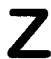
\includegraphics[keepaspectratio]{images/part001_5bbbde23.jpg}}

注意在条件 (i) 中并非如此：一个对 A 完全割的序列未必是 A-正则的 (习题 1)。

\begin{enumerate}
\def\labelenumi{\arabic{enumi})}
\setcounter{enumi}{1}
\tightlist
\item
  设 A 为环，J 为 A 的一个有限生成理想，p 为 A 的一个包含 J 的素理想。由 § 1, 第 3 节的定理 1 的推论 2，有

\[
\operatorname{prof} _ {A _ {\mathfrak {p}}} (J _ {\mathfrak {p}}; A _ {\mathfrak {p}}) \leqslant [ \kappa (\mathfrak {p}) \otimes_ {A} J: \kappa (\mathfrak {p}) ],
\]

且等号成立当且仅当 J 在 p 处完全割。
\end{enumerate}

设 J 异于 A 且由一个完全割序列 \((x_{1},\ldots,x_{r})\) 生成。则有 (§ 1, 第 3 节的命题 4 及上面的命题 1)

\[
\operatorname{prof} _ {A} (J; A) = \inf _ {\mathfrak {p} \in V (J)} \operatorname{prof} _ {A _ {\mathfrak {p}}} (J _ {\mathfrak {p}}; A _ {\mathfrak {p}}) = r.
\]

若进而 A 是 Noether 环，则有 \(\operatorname{codim}(\mathrm{V}(\mathrm{J}),\operatorname{Spec}(\mathrm{A}))\leqslant r\) (VIII, § 3, 第 3 节, 命题 4) 与 \(\operatorname{prof}_{\mathrm{A}}(\mathrm{J};\mathrm{A})\leqslant \operatorname{codim}(\mathrm{V}(\mathrm{J}),\operatorname{Spec}(\Lambda))\) (§ 1, 第 7 节, 命题 12)，从而最终有

\[
\operatorname{prof} _ {\mathrm{A}} (\mathrm{J}; \mathrm{A}) = r = \operatorname{codim} (\mathrm{V} (\mathrm{J}), \operatorname{Spec} (\mathrm{A})) = \operatorname{ht} (\mathrm{J}).
\]

\subsection{完全割理想的刻画}

设 A 为环，J 为 A 的理想。分次 A-模 \(\bigoplus_{n\in\mathbf{N}}J^{n}\) 具有一个自然的分次 A-代数结构，它由环 A 中的乘法导出；于是 J 到 \(J^{1}\) 的恒同映射扩张为分次 A-代数的一个满射同态，称为典范同态

\[
\alpha_ {J}: \mathsf {S} _ {A} (J) \longrightarrow \bigoplus_ {n \in N} J ^ {n}.
\]

通过向环 A/J 作纯量扩张，由 \(\alpha_{\mathrm{J}}\) 导出一个分次 A/J-代数的满射同态，也称为典范同态

\[
\beta_ {J}: \mathsf {S} _ {\mathrm{A} / J} (\mathrm{J} / \mathrm{J} ^ {2}) \longrightarrow \operatorname{gr} _ {J} (\mathrm{A}),
\]

\(\operatorname{avec} \mathrm{gr}_{\mathrm{J}}(\mathrm{A}) = \bigoplus_{n \in \mathbf{N}} \mathrm{J}^n / \mathrm{J}^{n+1}\) 。

定理 1.--- 设 A 为 Noether 环，J 为 A 的理想。下列条件等价：

\begin{enumerate}
\def\labelenumi{(\roman{enumi})}
\item
  理想 J 是完全割的；
\item
  理想 J 在每个极大理想 \(\mathfrak{m} \in V(J)\) 处都完全割；
\item
  A/J-模 J/J² 是投射的，且典范同态 \(\alpha_{J}: S_{\Lambda}(J) \longrightarrow \bigoplus_{n \in \mathbb{N}} J^{n}\) 是双射；
\item
  \(\Lambda/\mathrm{J}\) -模 \(\mathrm{J}/\mathrm{J}^2\) 是投射的，且典范同态 \(\beta_{\mathrm{J}}:\mathbf{S}_{\mathrm{A}/\mathrm{J}}(\mathrm{J}/\mathrm{J}^2)\longrightarrow\mathrm{gr}_{\mathrm{J}}(\mathrm{A})\) 是双射。
\end{enumerate}

(i)⇒(ii)：这是显然的。

(ii)⇒(iii)：设条件 (ii) 满足。只需证明：对 A 的每个极大理想 m，\(A_{m}/J_{m}\) -模 \(J_{m}/J_{m}^{2}\) 是自由的，且同态 \(\alpha_{J_{m}}: S_{A_{m}}(J_{m}) \longrightarrow \bigoplus_{n} J_{m}^{n}\) 是双射 (II, § 5, 第 2 节, 定理 1 及 § 3, 第 3 节, 定理 1)。但当 m 不属于 V(J) 时这些断言是显然的，因为此时有 \(J_{m} = A_{m}\)；而当 m 属于 V(J) 时，它们由 A, X, 第 160 页的定理 1 及第 161 页的注得出。

\begin{enumerate}
\def\labelenumi{(\roman{enumi})}
\setcounter{enumi}{2}
\tightlist
\item
  \(\Rightarrow\) (iv)：这是显然的。
\end{enumerate}

\((\mathrm{iv}) \Rightarrow (\mathrm{i})\)：设条件 (iv) 满足；设 \(\mathfrak{p}\) 为 A 的一个包含 J 的素理想。则 \(A_{\mathfrak{p}} / J_{\mathfrak{p}}\) -模 \(J_{\mathfrak{p}} / J_{\mathfrak{p}}^2\) 是自由的。设 \(\mathbf{x} = (x_1, \ldots, x_r)\) 为 \(J_{\mathfrak{p}}\) 的元素的一个序列，它提升 \(J_{\mathfrak{p}} / J_{\mathfrak{p}}^2\) 的一组基。序列 \(\mathbf{x}\) 生成 \(J_{\mathfrak{p}}\)（Nakayama 引理），且按构造满足命题 1 的条件 (iv)。于是理想 \(J_{\mathfrak{p}}\)（\(A_{\mathfrak{p}}\) 中的）是完全割的，即 J 在 \(\mathfrak{p}\) 处完全割。

注 1. 设理想 J 是完全割的；设 \((x_1, \ldots, x_r)\) 为 J 的元素的一个序列，使得对每个极大理想 \(\mathfrak{m} \in V(J)\)，\(x_i\) 在 J/mJ 中的典范像构成这个 A/m-向量空间的一组基。则 A/J-模 \(J/J^2\) 是自由的，且在 \(J/J^2\) 中 \(x_i\) 的典范像构成它的一组基：事实上只需验证：\(x_i\) 的像构成 \(A_{\mathfrak{m}}/J_{\mathfrak{m}}\) -模 \(J_{\mathfrak{m}}/J_{\mathfrak{m}}^2\) 的一组基（对每个 \(\mathfrak{m} \in V(J)\)） (II, § 3, 第 3 节, 定理 1)，而这由同上引文第 2 节的命题 5 与推论 2 得出，因为 \(A_{\mathfrak{m}}/J_{\mathfrak{m}}\) -模 \(J_{\mathfrak{m}}/J_{\mathfrak{m}}^2\) 是投射的 (定理 1)。

推论 1.--- 设 \(\widehat{\mathrm{A}}\) 为 A 关于 J-进拓扑的分离完备化，\(\widehat{\mathrm{J}} = \mathrm{J}\widehat{\mathrm{A}}\) 为 J 的分离完备化。为使理想 \(\widehat{\mathrm{J}}\)（\(\widehat{\mathrm{A}}\) 中的）完全割，必须且只需 A 的理想 J 完全割。

事实上，典范映射 \(\mathrm{gr}_{\mathrm{J}}(\mathsf{A}) \to \mathrm{gr}_{\widehat{\mathrm{J}}}(\widehat{\mathsf{A}})\) 是分次环的同构；因此只需应用判别法 (iv)。

更一般地：

推论 2.--- 设 ρ : A → B 为一个 Noether 环的同态，它使 B 成为平坦 A-模，并设 J 为 A 的理想。

\begin{enumerate}
\def\labelenumi{\alph{enumi})}
\item
  若 J 完全割，则 B 的理想 JB 完全割。
\item
  设 B 的理想 JB 完全割，且 \(\mathfrak{m} \in \mathrm{V}(\mathrm{J})\) 的每个极大理想都是 B 的某个极大理想的原像。则理想 J 完全割。例如当 B 是忠实平坦 A-模时就是这种情形。
\end{enumerate}

首先注意，由于 B 是平坦 A-模，\(J^n \otimes_A B\) 等同于 \(J^n B\)，且 \((J^n / J^{n+1}) \otimes_{A/J} (B/JB)\) 等同于 \(J^n B / J^{n+1} B\)（对每个整数 \(n \geqslant 0\)）。于是断言 a) 由判别法 (iii) 得出。在 b) 的假设下，A/J-模 B/JB 是忠实平坦的 (I, § 2, 第 7 节, 命题 8 的推论 2 及 § 3, 第 5 节, 命题 9)，且考虑到 I, § 3, 第 1 节, 命题 2 及第 6 节, 命题 12，J 依判别法 (iv) 完全割。最后的断言由 I, § 3, 第 5 节的命题 8 得出。

推论 3.-- 设 A 为 Noether 环，J 为 A 的完全割理想。若 A 是 Macaulay 环（相应地 Gorenstein 环），则 A/J 亦然。

事实上，设 m 为 A 的一个包含 J 的极大理想。理想 \(J_{m}\)（\(\Lambda_{m}\) 中的）由一个 \(A_{m}\) -正则序列生成；于是 \((A/J)_{m}\) 是 Macaulay 环（相应地 Gorenstein 环），依据是 § 2, 第 5 节的例 6（相应地 § 3, 第 9 节的例 2）。

注 2. — 称 Noether 环 A 为完全交环，如果对 A 的每个极大理想 m，完备局部环 \(\widehat{A_{m}}\) 同构于一个正则完备 Noether 局部环对一个完全交理想的商。由上面的推论 3 及 § 3, 第 8 节的命题 12 的推论 2 得出，这样的环是 Gorenstein 环。

\subsection{完全交理想与正则环}

命题 2.--- 设 A 为 Noether 环。下列条件等价：

\begin{enumerate}
\def\labelenumi{(\roman{enumi})}
\item
  A 是正则的；
\item
  A 的每个极大理想都完全割；
\item
  A 的每个使 A/J 正则的理想 J 都完全割。
\end{enumerate}

(i)⇒(iii)：设环 A 正则；设 J 为 A 的理想使 Λ/J 正则，并设 p 为 A 的一个包含 J 的素理想。则局部环 \(A_{p}\) 与 \(A_{p}/J_{p}\) 都正则，于是 \(J_{p}\) 由一个对 \(A_{p}\) 完全割的序列生成 (VIII, § 5, 第 3 节, 推论 2 与命题 2)，这就意味着 J 在 p 处完全割。

\begin{enumerate}
\def\labelenumi{(\roman{enumi})}
\setcounter{enumi}{2}
\tightlist
\item
  (ii)：这是显然的，因为域是正则环。
\end{enumerate}

(ii)⇒(i)：设 m 为 A 的一个极大理想；在假设 (ii) 下，极大理想 mA \(_{m}\)（Λ \(_{m}\) 中的）由一个对 A \(_{m}\) 完全割的序列生成，因此 Λ \(_{m}\) 正则 (VIII, § 5, 第 2 节, 定理 1)。于是 A 正则。

命题 3.--- 设 A 为 Noether 环，J 为 A 的理想且 A/J 正则。下列条件等价：

\begin{enumerate}
\def\labelenumi{(\roman{enumi})}
\item
  理想 J 完全割；
\item
  对 A 的每个包含 J 的素理想（相应地极大理想）p，环 A \(_{p}\) 都正则；
\item
  A 关于 J-进拓扑的分离完备化是正则的。
\end{enumerate}

由定理 1，条件 (i) 意味着：对 A 的每个包含 J 的素理想（相应地极大理想）p，理想 \(J_{p}\)（局部环 \(A_{p}\) 中的）由一个对 \(A_{p}\) 完全割的序列生成。由于按假设 \(A_{p}/J_{p}\) 正则，后一条件等价于 \(A_{p}\) 正则 (VIII, § 5, 第 3 节, 命题 2 及其推论 2)；这就证明了 (i) 与 (ii) 的等价性。(ii) 与 (iii) 的等价性由 § 4, 第 2 节, 命题 4 的推论 3 得出。

命题 4.--- 设 A 为正则环，J 为 A 的理想，\(A_{0}\) 为 A 的子环且典范同态 \(A_{0} \rightarrow A/J\) 是双射的。

\begin{enumerate}
\def\labelenumi{\alph{enumi})}
\item
  理想 J 完全割，\(A_{0}\) -模 \(J/J^{2}\) 是有限型投射的，且环 \(A_{0}\) 正则。
\item
  设 \(\varphi: J/J^{2} \to J\) 为一个 \(A_{0}\) -线性截面（对典范满射 \(J \to J/J^{2}\)）。\(A_{0}\) -代数同态 \(\mathsf{S}_{A_{0}}(J/J^{2}) \longrightarrow A\)（它扩张 \(\varphi\)）扩张为分次环 \(\mathsf{S}_{A_{0}}(J/J^{2})\) 的完备化到 \(A\) 关于 \(J\) -进拓扑的分离完备化上的一个同构。
\end{enumerate}

\begin{enumerate}
\def\labelenumi{\alph{enumi})}
\item
  设 \(\mathfrak{p}\) 为 A 的一个包含 J 的素理想。我们有 \(\mathfrak{p} = (\mathfrak{p} \cap A_0) \oplus J\)，从而 \(\mathfrak{p}^2 = (\mathfrak{p} \cap A_0)^2 \oplus \mathfrak{p}J\)，故 \(\mathfrak{p}^2 \cap J = \mathfrak{p}J\)。设 \(i\) 为 \(J\) 到 \(\mathfrak{p}\) 中的典范单射。由前所述，映射 \(i \otimes 1_{A/p}: J \otimes_A A/p \longrightarrow \mathfrak{p} \otimes_A A/p\) 是单射的，对 \(i_{\mathfrak{p}} \otimes 1_{\kappa(\mathfrak{p})}: J_{\mathfrak{p}} \otimes_{A_{\mathfrak{p}}} \kappa(\mathfrak{p}) \longrightarrow \mathfrak{p}A_{\mathfrak{p}} \otimes_{A_{\mathfrak{p}}} \kappa(\mathfrak{p})\) 亦然。Nakayama 引理蕴含：理想 \(J_{\mathfrak{p}}\)（\(A_{\mathfrak{p}}\) 中的）由正则局部环 \(A_{\mathfrak{p}}\) 的一个坐标系的一个子集生成。根据 VIII, § 5, 第 3 节的命题 2，环 \(A_{\mathfrak{p}}/J_{\mathfrak{p}}\) 正则且理想 \(J_{\mathfrak{p}}\) 完全割。于是 \(J\) 完全割，环 \(A_0\) 同构于 \(A/J\) 故正则，且由定理 1（第 2 节），\(A_0\) -模 \(J/J^2\) 是有限型投射的。
\item
  由定理 1，典范同态 \(\beta_{\mathrm{J}}: \mathsf{S}_{\mathrm{A}_{0}}(\mathrm{J}/\mathrm{J}^{2}) \longrightarrow \mathrm{gr}_{\mathrm{J}}(\mathrm{A})\) 是双射的。设 \(f: \mathsf{S}_{\mathrm{A}_{0}}(\mathrm{J}/\mathrm{J}^{2}) \longrightarrow \mathrm{A}\) 为 \(\mathrm{A}_{0}\) -代数同态，它扩张 \(\mathrm{A}_{0}\) -线性映射 \(\varphi: \mathrm{J}/\mathrm{J}^{2} \longrightarrow \mathrm{J}\)。若给 A 赋以 J-进滤链，并给 \(\mathsf{S}_{\mathrm{A}_{0}}(\mathrm{J}/\mathrm{J}^{2})\) 赋以与其分次相伴的滤链，则 \(\beta_{\mathrm{J}}\) 等同于由 \(f\) 通过取相伴分次对象得到的同态。于是断言 b) 由 III, § 2, 第 8 节, 定理 1 的推论 3 得出。
\end{enumerate}

\subsection{分次正则环}

设 \(A_{0}\) 为环，P 为一个 \(A_{0}\) 上的 N 型分次模且次数 \textgreater{} 0。用 A 表示环 \(\mathsf{S}_{\mathrm{A}_{0}}(\mathrm{P})\)；A 上存在唯一的 N-分次结构，使 \(A_{0}\) 的次数为 0 且 P 是 A 上的一个子 \(A_{0}\) -分次模。用 \(A_{+}\) 表示 A 的理想 \(\bigoplus_{n>0} A_{n}\)。则典范映射 \(P \longrightarrow A_{+}/A_{+}^{2}\) 是 \(A_{0}\) -分次模的同构 (参见 A, III, 第 76 页, 命题 10)。

若 \(A_{0}\) -模 P 是分次自由的 (A, II, 第 167 页, 注 3)，且 \((x_{i})_{i\in I}\) 是由齐次元素组成的 P 的一组基，则 \(A_{0}\) -分次代数 \(\mathbf{S}_{\Lambda_{0}}(\mathbf{P})\) 同构于多项式代数 \(\mathrm{A}_{0}[(\mathrm{X}_{i})_{i\in I}]\)，后者赋以使每个 \(X_{i}\) 为次数 \(\deg(x_{i})\) 的齐次元素的分次结构。我们称每个 N 型 \(A_{0}\) -分次代数为 \(A_{0}\) -分次多项式代数，如果它同构于前述形状的一个 \(A_{0}\) -分次代数。

当环 \(\Lambda_0\) 正则且 \(\mathrm{A}_0\) -模 P 是有限生成投射的时，环 \(\mathsf{S}_{\mathrm{A}_0}(\mathrm{P})\) 正则 ( \(\S 4\) , 见第 2 节, 命题 4 的推论 4)。反之：

定理 2.--- 设 A 为正则环，N 型分次的。由 A 中次数为 0 的元素组成的环 A₀ 是正则的；存在一个次数 \textgreater{} 0 的有限生成分次投射 A₀-模 P，使 A 作为分次 A₀-代数同构于 \(S_{A_{0}}(P)\)。

用 P 表示 \(A_{0}\) 分次模 \(A_{+}/A_{+}^{2}\)。由第 3 节的命题 4，环 \(A_{0}\) 正则且 \(A_{0}\) -模 P 是投射的且有限生成的。于是 P 的齐次分量都是投射的，且存在一个 \(A_{0}\) -线性截面 \(\varphi: P \to A_{+}\)（它是次数为 0 的分次映射，作用于典范满射 \(A_{+} \to P\)）。设 \(f: S_{\mathrm{A}_{0}}(\mathrm{P}) \longrightarrow \Lambda\) 为 \(A_{0}\) -代数同态，它扩张 \(\varphi\)。由命题 4，f 扩张为 \(\mathbf{S}_{\mathrm{A}_{0}}(\mathrm{P})\) 关于 \(\mathbf{S}_{\mathrm{A}_{0}}(\mathrm{P})_{+}\) -进拓扑的分离完备化到 A 关于 \(A_{+}\) -进拓扑的分离完备化上的一个同构。因此 f 是单射的，且它的像在 A 中对 \(A_{+}\) -进拓扑是稠密的。但由于 A 的齐次分量上的诱导拓扑是离散的，且 f 的像是一个分次子模，这就蕴含 f 是双射的。

推论 1. - 设 B 为正则环，带正次数的分次环。假设每个有限型投射 \(\mathbf{B}_0\) -模都是自由的。

\begin{enumerate}
\def\labelenumi{\alph{enumi})}
\item
  环 B \(_{0}\) 是整环且正则，且 B \(_{0}\) -代数 B 是一个 B \(_{0}\) 分次多项式代数，有限型的。
\item
  设 A 为 B 的一个分次子环使 \(A_{0} = B_{0}\)，且 B 是有限生成 A-模。下列条件等价：
  \begin{enumerate}
  \def\labelenumii{(\roman{enumii})}
  \item
    A-模 B 是分次自由的；
  \item
    A-模 B 是平坦的；
  \item
    A 是一个 \(A_{0}\) 分次多项式代数，有限型的。
  \end{enumerate}
\end{enumerate}

由定理 2，环 B₀ 正则，从而是正则整环的乘积 (§ 4, 第 2 节, 例 2)。对 B₀ 的每个幂等元 e，B₀-模 B₀e 是投射的，从而是自由的，这蕴含 e = 0 或 1；于是 B₀ 是整环。于是断言 a) 由定理 2 及有限型分次投射 B₀-模是分次自由的这一事实得出。

我们来证明 b)。

\begin{enumerate}
\def\labelenumi{(\roman{enumi})}
\item
  \(\Leftrightarrow\) (ii)：有限型分次平坦 \(A_0\) -模都是分次自由的 (II, § 5, 第 2 节, 定理 1 的推论 2)。于是 (i) 与 (ii) 的等价性由 A, X, 第 144 页, 命题 8 得出。
\item
  \(\Leftrightarrow\) (iii)：由于 B 在 A 上是整的且是有限生成 A \(_0\) -代数，A 是有限型 A \(_0\) -代数 (V, § 1, 第 9 节, 引理 5)，从而是 Noether 环。于是 (ii) 与 (iii) 的等价性由 § 4, 第 5 节的命题 8 的推论以及应用到 A 的 a) 得出。
\end{enumerate}

推论 2.- 设 \(k\) 为域，B 为一个 \(k\) -分次多项式代数，有限型的，A 为 B 的一个分次子代数。下列条件等价：

\begin{enumerate}
\def\labelenumi{(\roman{enumi})}
\item
  B 是分次自由 Λ-模；
\item
  B 是平坦 A-模；
\item
  有 \(\mathrm{Tor}_1^\Lambda (k,\mathbf{B}) = 0\)；
\item
  代数 A 是一个有限生成分次多项式 k-代数，且 A 的每个由齐次元素组成的代数自由生成序列都是 B-正则的。
\end{enumerate}

蕴含关系 (i) \(\Rightarrow\) (ii) 与 (ii) \(\Rightarrow\) (iii) 是显然的，而蕴含关系 (iii) \(\Rightarrow\) (i) 由 \(\Lambda\) , X, 第 144 页, 命题 8 a) 得出。

(i)⇒(iv)：由于环 B 正则且在 A 上忠实平坦，环 A 由 I, § 3, 第 6 节的命题 11 是 Noether 的，且由 § 4, 第 5 节的命题 8 是正则的，从而是一个分次多项式 k-代数 (推论 1, a))。A 的每个代数自由生成序列都是 A-正则的 (A, X, 第 158 页, 例)，从而由于 B 在 A 上平坦而是 B-正则的。

((iv) \(\Rightarrow\) (iii))：设条件 (iv) 满足，并设 x 为 A 的一个由齐次元素组成的代数自由生成序列。由于序列 x 是 A-正则的，它对 A 是完全割的 (A, X, 第 157 页, 命题 5)，于是 A-模 \(\mathrm{Tor}_{1}^{\mathrm{A}}(k,\mathrm{B})\) 同构于 \(\mathrm{H}_{1}(\mathbf{x},\mathrm{B})\) (A, X, 第 159 页, 注 3)；但后者为零，因为序列 x 是 B-正则的。

推论 1 与推论 2 蕴含 LIE, V, § 5, 第 5 节的引理 5。

\subsection{正则序列与纯量扩张}

命题 5.--- 设 \(\mathfrak{p}: A \to B\) 为 Noether 局部环的局部同态，N 为有限生成 B-模，\(\mathbf{x} = (x_1, \ldots, x_r)\) 为 \(\mathfrak{m}_B\) 的元素的一个序列，\(u: A[T_1, \ldots, T_r] \longrightarrow B\) 为唯一的 A-代数同态，使 \(u(T_i) = x_i\)（对 \(i = 1, \ldots, r\)）。下列条件等价：

\begin{enumerate}
\def\labelenumi{(\roman{enumi})}
\item
  同态 u 使 N 成为平坦的 A{[}T \(_{1}\) ,\ldots{} ,T \(_{r}\) {]}-模；
\item
  A-模 N 是平坦的，且对每个 A-模 M，序列 x 是 M ⊗A N-正则的；
\item
  A-模 N 是平坦的且序列 x 是 \(\kappa_{A} \otimes_{A} N\)-正则的；
\item
  A-模 N/(x₁N + \ldots{} + xᵣN) 是平坦的且序列 x 是 N-正则的。
\end{enumerate}

(i)⇒(ii)：令 \(\mathbf{T} = (\mathrm{T}_{1}, \ldots, \mathrm{T}_{r})\)。设 A{[}T{]}-模 N 是平坦的。由于 A{[}T{]} 在 A 上平坦，A-模 N 是平坦的 (I, § 2, 第 7 节, 命题 8 的推论 3)。设 M 为 A-模。序列 T 显然是 M{[}T{]}-正则的，从而是 M{[}T{]} ⊗\_\{A{[}T{]}\} N-正则的，因为 N 在 A{[}T{]} 上平坦。而 A{[}T{]}-模 M{[}T{]} ⊗\_\{A{[}T{]}\} N 等同于 M ⊗\_\{A\} N，比为 T\_i 的同态对应于自同态 1\_M ⊗ (x\_i)\_N。因此条件 (ii) 满足。

\begin{enumerate}
\def\labelenumi{(\roman{enumi})}
\setcounter{enumi}{1}
\tightlist
\item
  \(\Rightarrow\) (iii)：这是显然的。
\end{enumerate}

(iii)⇒(iv)：这由 § 1, 第 6 节的命题 10 得出。

(iv)⇒(i)：用 t 表示 A{[}T{]} 中由 T 生成的理想。(A{[}T{]}/t)-模 N/tN 按假设是平坦的，且 N 对 t 是理想分离的 (III, § 5, 第 4 节, 命题 2)。为证明 N 在 A{[}T{]} 上平坦，鉴于同上引文第 2 节的定理 1，只需证明 A-模 \(\operatorname{Tor}_{1}^{A{[}T{]}}(A{[}T{]}/t,N)\) 为零。但由于序列 T 是 A{[}T{]}-正则的，该模同构于 \(\mathrm{H}_{1}(T,N)\) (A, X, 第 159 页, 注 3)，而它为零，因为序列 T 是 N-正则的（同上引文, 第 157 页, 命题 5）。

推论. 设 \(k\) 为域，\(\Lambda\) 为一个 \(k\) 上的 Noether 局部代数，\(\mathbf{x} = (x_1, \ldots, x_r)\) 为 \(\mathfrak{m}_{\mathrm{A}}\) 的元素的一个序列，M 为 \(\Lambda\) 上的有限型模。用 \(\widehat{\mathrm{A}}\) 和 \(\widehat{\mathrm{M}}\) 表示 A 和 M 关于其 ( \(x_1\mathrm{A} + \ldots + x_r\mathrm{A}\) -进拓扑的完备化；用 \(u: k[\mathrm{T}_1, \ldots, \mathrm{T}_r] \longrightarrow \mathrm{A}\) 表示唯一的 \(k\) -代数同态，使 \(u(\mathrm{T}_i) = x_i\)（对 \(i = 1, \ldots, r\)），并用 \(\hat{u}: k[[\mathrm{T}_1, \ldots, \mathrm{T}_r]] \longrightarrow \widehat{\mathrm{A}}\) 表示扩张它的唯一连续同态。下列条件等价：

\begin{enumerate}
\def\labelenumi{(\roman{enumi})}
\item
  序列 x 是 M-正则的；
\item
  同态 u 使 M 成为平坦的 \(k[T_{1},\ldots,T_{r}]\) -模；
\item
  同态 \(\hat{u}\) 使 \(\hat{M}\) 成为平坦的 \(k[[T_{1},\ldots,T_{r}]]\) -模。
\end{enumerate}

(i) 与 (ii) 的等价性由命题 5 的条件 (i) 与 (iv) 的等价性得出；(ii) 与 (iii) 的等价性由 III, § 5, 第 4 节, 命题 4 得出。

这些结果使我们能在两个重要情形刻画 Macaulay 模。用 \(\Lambda\) 表示一个 Noether 局部环，M 为一个有限生成 A-模。说 \(\Lambda\) -模 M 是 Macaulay 的等价于说 \(\widehat{A}\) -模 \(\widehat{M}\) 是 Macaulay 的 ( \(\S\) 2, 第 7 节, 命题 8 的推论 4)。以下我们总假设 Noether 局部环 A 是完备的。

\begin{enumerate}
\def\labelenumi{\arabic{enumi})}
\tightlist
\item
  先设 A 具有一个子域；于是它具有一个代表域 \(k\) (IX, § 3, 第 3 节, 定理 1)。设 \((x_{1},\ldots ,x_{r})\) 为对 M 的一个极大割序列；用 \(u:k[[\mathrm{T}_{1},\dots ,\mathrm{T}_{r}]]\longrightarrow \Lambda\) 表示唯一的连续同态，使 \(u(\mathrm{T}_i) = x_i\)（对 \(i = 1,\dots ,r\)）。由 IX, § 2, 第 5 节的引理 4 b) 及 VIII, § 3, 第 2 节的注 1，A/Ann(M) 是有限型 \(k[[\mathrm{T}_{1},\dots ,\mathrm{T}_{r}]]\) -模，从而 M 是有限型 \(k[[\mathrm{T}_{1},\dots ,\mathrm{T}_{r}]]\) -模。这样，下列条件等价：
  \begin{enumerate}
  \def\labelenumii{(\roman{enumii})}
  \item
    \(k[[\mathrm{T}_1,\dots ,\mathrm{T}_r]]\) -模 M 是自由的；
\item
    A-模 M 是 Macaulay 的。
\end{enumerate}

事实上，说 M 是 Macaulay A-模等价于说序列 \((x_{1},\ldots,x_{r})\) 是 M-正则的 (§ 2, 第 3 节, 定理 1)。由上面的推论，后一条件意味着模 M 在 \(k[[T_{1},\ldots,T_{r}]]\) 上平坦，等价地，由于它有限生成，它是自由的。

\item
  设 A 的剩余域 \(\kappa_{\Lambda}\) 的特征为 \(p > 0\)，且有 \(\dim(M/pM) < \dim(M)\) 。设 \((x_1, \ldots, x_r)\) 为对 M/pM 的一个极大割序列，于是 \((p1_{\mathrm{A}}, x_1, \ldots, x_r)\) 是对 M 的极大割序列。设 C 为一个 \(p\) -环，长度 \(+\infty\)，其剩余域为 \(\kappa_{\Lambda}\) (IX, § 2, 第 3 节, 命题 5)。存在一个从 C 到 A 中的同态 \(u_0\)，它在剩余域上诱导恒同；设 \(u: \mathrm{C}[[\mathrm{T}_1, \ldots, \mathrm{T}_r]] \longrightarrow \mathrm{A}\) 为扩张 \(u_0\) 且把 \(\mathrm{T}_i\) 映到 \(x_i\)（对每个 \(i\)）的唯一同态。与前面一样，由同上引文第 5 节的引理 4 得出，\(u\) 使 M 成为有限型 \(\mathrm{C}[[\mathrm{T}_1, \ldots, \mathrm{T}_r]]\) -模。下列条件等价：
  \begin{enumerate}
  \def\labelenumii{(\roman{enumii})}
\item
    C{[}{[}T1, \ldots, Tr{]}{]}-模 M 是自由的；
\item
    A-模 M 是 Macaulay 的。
\end{enumerate}

事实上，条件 (ii) 等价于说序列 \((x_{1},\ldots,x_{r})\) 是 M-正则的，且比为 p 的同态在 \(\mathrm{M}/(x_{1}\mathrm{M}+\ldots+x_{r}\mathrm{M})\) 中是单射的 (§ 2, 第 3 节, 定理 1)。但后一条件意味着 C-模 \(\mathrm{M}/(x_{1}\mathrm{M}+\ldots+x_{r}\mathrm{M})\) 是无挠的，从而是平坦的 (Λ, X, 第 9 页, 例 7)。于是，鉴于命题 5 的 (iv)⇔(i)，条件 (ii) 等价于模 M 在 \(C[T_{1},\ldots,T_{r}]\) 上平坦，或等价地 (III, § 5, 第 4 节, 命题 4)，\(C[[T_{1},\ldots,T_{r}]]\) -模 M 是平坦的，即由于它有限生成而是自由的。

\end{enumerate}

\subsection{完全交理想与纯量扩张}

命题 6. - 设 \(\rho: A \to B\) 为 Noether 环的同态，J 为 B 的理想。下列条件等价：

\begin{enumerate}
\def\labelenumi{(\roman{enumi})}
\item
  A-模 B/J 是平坦的且理想 J 完全割。
\item
  对每个 \(\mathfrak{q} \in \mathrm{V}(\mathrm{J})\)，A-模 \(\mathrm{B}_{\mathfrak{q}}\) 是平坦的，且对每个 A-代数 \(\mathrm{A}'\)（使环 \(\Lambda' \otimes_{\mathrm{A}} \mathrm{B}\) 为 Noether 环的），理想 \(\mathrm{J}(\mathrm{A}' \otimes_{\mathrm{A}} \mathrm{B})\)（\(\mathrm{A}' \otimes_{\mathrm{A}} \mathrm{B}\) 中的）都完全割；
\item
  对 B 的每个包含 J 的极大理想 n，A-模 \(B_{n}\) 是平坦的，且理想 \(\mathrm{J}(\kappa(\rho^{-1}(\mathfrak{n}))\otimes_{\mathrm{A}}\mathrm{B}_{\mathfrak{n}})\)（\(\kappa(\rho^{-1}(\mathfrak{n}))\otimes_{\mathrm{A}}\mathrm{B}_{\mathfrak{n}}\) 中的）完全割。
\end{enumerate}

由第 2 节的定理 1，条件 (i) 等价于条件 (i′)（相应地 (i′\,），即下列条件：

(i')（相应地 (i'\,）对 B 的每个包含 J 的素理想（相应地极大理想）q，\(A_{p^{-1}(q)^{-}}\) -模 \(B_{q}/J_{q}\) 是平坦的，且理想 \(J_{q}\)（\(B_{q}\) 中的）由一个 \(B_{q}\) -正则序列生成。

\((i') \Rightarrow (ii)\) ：设 \((i')\) 成立。设 \(A'\) 为一个 A-代数，使环 \(B' = A' \otimes_A B\) 是 Noether 的。设 \(q\) 为 B 的一个包含 \(J\) 的素理想；令 \(p = \rho^{-1}(q)\) 。由于 \(B_q'\) 等同于 \(A_p' \otimes_{A_p} B_q\)，由命题 5 的蕴含关系 \((iv) \Rightarrow (ii)\)（ \(n^o 5\) ）得出：理想 \(JB_q'\)（\(B_q'\) 中的）由一个 \(B_q'\) -正则序列生成，且 \(B_q\) 在 \(A_p\) 上平坦，从而在 \(A\) 上平坦。此外，对每个素理想 \(r\)（\(B'\) 中的，包含 \(JB'\)），令 \(q\) 为 \(r\) 在 B 中的原像（它包含 \(J\)），且 \(B_r'\) 等同于 \(B_q'\) 的一个分式环。于是 \(JB_r'\) 是 \(B_r'\) 的完全割理想，\(JB'\) 是 \(B'\) 的完全割理想。

\begin{enumerate}
\def\labelenumi{(\roman{enumi})}
\setcounter{enumi}{1}
\tightlist
\item
  \(\Rightarrow\) (iii)：这是显然的。
\end{enumerate}

(iii)⇒ (i'\,)：设 (iii) 成立。设 n 为 B 的一个包含 J 的极大理想；令 m = ρ \(^{-1}\) (n)。设 x 为 Jn 的元素的一个序列，其像在 Jn/nJn 中构成这个 κ(n)-向量空间的一组基。序列 x 生成 Jn；由第 1 节的命题 1，它是 (κ(m) ⊗A Bn)-正则的。由于 Am-模 Bn 按假设是平坦的，由命题 5 的蕴含关系 (iii)⇒ (iv) 得出条件 (i'\,') 满足。

注 1.--- 设命题 6 的等价条件满足。由于 B/J 在 A 上平坦，对每个 A-代数 A'，A'-模的典范序列

\[
0 \rightarrow \Lambda^ {\prime} \otimes_ {A} J \longrightarrow A ^ {\prime} \otimes_ {A} B \longrightarrow A ^ {\prime} \otimes_ {A} (B / J) \rightarrow 0
\]

因此是正合的，且典范同态 \(A'\otimes_A J \longrightarrow J(A'\otimes_A B)\) 是双射的。

\section{正则代数中的纯量扩张}

\subsection{本质有限型代数}

设 \(k\) 为环。设 A 为一个 \(k\) -代数，\(\mathbf{x} = (x_i)_{i \in I}\) 为 A 的元素的一个族；用 \(\mathbf{A}'\) 表示由 \(x_i\) 生成的 A 的子代数。若族 \(\mathbf{x}\) 满足下列条件，则称它为 \(k\) -代数 A 的一个本质生成族：对 A 的每个元素 \(a\)，存在一个元素 \(s\)（属于 \(\mathbf{A}'\) 且在 A 中可逆），使 \(sa\) 属于 \(\mathbf{A}'\)。这等价于说：对每个 \(a \in \mathbf{A}\)，存在多项式 P 和 Q（在 \(k[(\mathrm{X}_i)_{i \in I}]\) 中），使 \(\mathrm{Q}(\mathbf{x})\) 在 A 中可逆且有 \(a = \mathrm{P}(\mathbf{x})\mathrm{Q}(\mathbf{x})^{-1}\) 。

我们将称一个 \(k\) -代数 A 是本质有限型的，如果它具有一个有限本质生成族。这等价于说：存在一个有限型的 \(k\) -代数 A' 和 A' 的一个乘性子集 S，使 \(k\) -代数 A 同构于 \(\mathrm{S}^{-1}\mathrm{A}'\) 。

例.--- 1) 说域 K 的扩张 L 是一个本质有限生成 K-代数，意味着它是 A, V, 第 11 页, 定义 2 意义下的有限生成扩张。K-代数 L 是有限型的，仅当它是 K 的有限次扩张 (V, § 3, 第 4 节, 定理 3 的推论 3)。

\begin{enumerate}
\def\labelenumi{\arabic{enumi})}
\setcounter{enumi}{1}
\tightlist
\item
  为使一个 \(k\) -代数是局部的且本质有限型的，必须且只需它同构于一个 \(k\) -代数（形如 \(\mathsf{A}_{\mathfrak{p}}\)），其中 A 是一个有限生成 \(k\) -代数，\(\mathfrak{p}\) 是 A 的素理想 (参见 II, § 2, 第 5 节, 命题 11 (iii))。
\end{enumerate}

命题 1. - 若环 k 是 Noether 的，则每个本质有限生成 k-代数都是 Noether 环。

这由 III, § 2, 第 10 节, 定理 2 的推论 3 及 II, § 2, 第 4 节, 命题 10 的推论 2 得出。

由定义，我们导出下列性质：

命题 2.--- a) 本质有限型 k-代数的每个商代数都是本质有限型的。

\begin{enumerate}
\def\labelenumi{\alph{enumi})}
\setcounter{enumi}{1}
\item
  本质有限生成 k-代数的每个分式环都是本质有限生成 k-代数。
\item
  有限个本质有限型 \(k\) -代数的乘积 \(k\) -代数是本质有限型的。
\item
  设 \(k \to k'\) 为环同态；对每个本质有限型 \(k\) -代数 A，\(k'\) -代数 \(A_{(k')} = k' \otimes_k \Lambda\) 都是本质有限型的。
\end{enumerate}

推论.- 设 A 为本质有限型 \(k\) -代数，B 为 Noether 的 \(k\) -代数。则环 \(\mathrm{A} \otimes_k \mathrm{B}\) 是 Noether 的。

事实上，它是一个本质有限型 B-代数 (命题 2, d))，于是应用命题 1。

命题 3. 设 \(k\) 为环，A 为一个线性拓扑化的形式平滑 \(k\) -代数，B 为 A-代数。若 A 在 \(k\) 上本质有限型且 B 在 A 上本质有限型，则 B 在 \(k\) 上本质有限型。

设 \(\rho: A \to B\) 为典范映射。设 \(x = (x_i)_{i \in I}\) 为 \(k\) -代数 \(A\) 的一个有限本质生成族，\(A'\) 为它生成的子代数；设 \(y = (y_j)_{j \in J}\) 为 \(A\) -代数 \(B\) 的一个有限本质生成族。设 \(B'\) 为子 \(k\) -代数（\(B\) 中的），由 \(\rho(x_i)\) 与 \(y_j\) 生成。设 \(b \in B\)；按假设存在多项式 \(P\) 和 \(Q\)（在 \(A[(Y_j)_{j \in J}]\) 中），使 \(Q(y)\) 在 \(B\) 中可逆且有 \(Q(y)b = P(y)\) 。\(P\) 和 \(Q\) 的非零系数只有有限多个；存在多项式 \(R \in k[(X_i)_{i \in I}]\)，使 \(R(x)\) 在 \(A\) 中可逆且 \(R(x)P\) 和 \(R(x)Q\) 属于 \(A'[[(Y_j)_{j \in J}]\) 。于是 \(\rho(R(x))Q(y)\) 在 \(B\) 中可逆，并且有

\[
\rho (\mathrm{R} (\mathbf {x})) \mathrm{Q} (\mathbf {y}) b = \rho (\mathrm{R} (\mathbf {x})) \mathrm{P} (\mathbf {y}) \in \mathrm{B} ^ {\prime}.
\]

于是元素 \(\rho(x_i)\)（对 \(i \in I\)）与 \(y_j\)（对 \(j \in J\)）构成 \(k\) -代数 B 的一个本质有限生成族。

推论. -- 两个本质有限型 k-代数的张量积是本质有限型 k-代数。

事实上，设 A 和 B 为两个本质有限生成 k-代数。则 \(A \otimes_{k} B\) 在 A 上本质有限型 (命题 2, d))，从而在 k 上本质有限型 (命题 3)。

\subsection{Macaulay 代数或 Gorenstein 代数的张量积}

命题 4. 设 k 为域，A 为本质有限生成 k-代数，B 为 k-代数。

\begin{enumerate}
\def\labelenumi{\alph{enumi})}
\item
  若 A 和 B 是 Macaulay 环，则 A ⊗k B 亦然。
\item
  若 A 和 B 是 Gorenstein 环，则 \(\Lambda\otimes_{k}\mathrm{B}\) 亦然。
\end{enumerate}

设 A 和 B 是 Macaulay（相应地 Gorenstein）环，我们来证明 \(A \otimes_{k} B\) 亦然。环 \(A \otimes_{k} B\) 是 Noether 的 (第 1 节, 命题 2 的推论)。A-模 \(A \otimes_{k} B\) 是自由的，从而是平坦的。由 § 2, 第 7 节的命题 10（相应地 § 3, 第 8 节的命题 12 的推论 1），只需证明：对 A 的每个素理想 p，\(\kappa(\mathfrak{p}) \otimes_{k} B\) 都是 Macaulay 环（相应地 Gorenstein 环）。由于扩张 \(\kappa(\mathfrak{p})\) 在 k 上是有限型的 (第 1 节, 命题 2 及例 1)，我们于是归结为证明 k-代数 A 是 k 的有限生成扩张 K 这一情形的命题。

设 \((t_{1},\ldots,t_{n})\) 为 K 在 k 上的一个超越基，于是 K 是纯扩张 \(k^{\prime}=k(t_{1},\ldots,t_{n})\) 的有限次扩张 (A, V, 第 112 页, 命题 17)。环 \(B^{\prime}=k^{\prime}\otimes_{k}B\) 同构于多项式环 \(B[T_{1},\ldots,T_{n}]\) 的一个分式环，从而由 § 2, 第 7 节的命题 10 的推论 2（相应地 § 3, 第 8 节的命题 12 的推论 3）是 Macaulay（相应地 Gorenstein）环。由于 \(K\otimes_{k}B\) 等同于 \(K\otimes_{k^{\prime}}B^{\prime}\)，我们归结为证明 K 是 k 的有限次扩张时断言 a) 和 b)。

环 K ⊗k B 此时是一个有限秩自由 B-模，从而是 Macaulay B-模。由 § 2, 第 6 节的命题 8 的推论 1，它是 Macaulay 环，这就证明了 a)。现在设 B 是 Gorenstein 环。存在 K 的子扩张 K \(_{i}\)（0 ≤ i ≤ m）：

\[
k = \mathrm{K} _ {0} \subset \mathrm{K} _ {1} \subset \dots \subset \mathrm{K} _ {m} = \mathrm{K}
\]

使 \(K_{i}\) 是 \(K_{i-1}\) -单生成代数（对 \(i = 1, \ldots, m\)），而这使我们能归结到 k 的扩张 K 是（有限次的）单生成的情形。典范同态 \(B \to K \otimes_{k} B\) 使 \(K \otimes_{k} B\) 成为平坦 B-代数，且对每个 \(\mathfrak{q} \in \operatorname{Spec}(B)\)，环 \((\mathrm{K} \otimes_{k} \mathrm{B}) \otimes_{\mathrm{B}} \mathfrak{k}(\mathfrak{q})\)（同构于 \(K \otimes_{k} \mathfrak{k}(\mathfrak{q})\)）是 \(\mathfrak{k}(\mathfrak{q})\) -单生成代数，从而是 Gorenstein 环 (§ 3, 第 9 节, 例 5)。于是 \(K \otimes_{k} B\) 是 Gorenstein 环 (§ 3, 第 8 节, 命题 12 的推论 1)，这就完成了 b) 的证明。

推论 1.--- 设 \(k\) 为域，K 为 \(k\) 的扩张，\(\Lambda\) 为本质有限型 \(k\) -代数。为使 \(\mathrm{A}_{(\mathrm{K})}\) 是 Macaulay 环（相应地 Gorenstein 环），必须且只需 A 亦然。

若 A 是 Macaulay（相应地 Gorenstein）环，则由命题 4，\(\mathrm{A}_{(\mathrm{K})}\) 亦然。由于 \(\mathrm{A}_{(\mathrm{K})}\) 是忠实平坦 A-模，逆命题由 § 2, 第 7 节的命题 10（相应地 § 3, 第 8 节的命题 12 的推论 1）得出。

推论 2.--- 设 k 为 Noether 环，A 和 B 为 k-代数。假设 A 在 k 上平坦且本质有限型。若 A 和 B 是 Macaulay 环（相应地 Gorenstein 环），则 A ⊗k B 是 Macaulay 环（相应地 Gorenstein 环）。

先设 B 是域；用 \(\varphi\) 表示从 \(k\) 到 B 中的典范同态，用 \(\mathfrak{r}\) 表示它的核。同态 \(\varphi\) 诱导一个从分式域 \(\kappa(\mathfrak{r})\)（\(k/\mathfrak{r}\) 的）到 B 中的同态。于是 A \(\otimes_{k}\) B 等同于 (A \(\otimes_{k}\) K(r)) \(\otimes_{\kappa(\mathfrak{r})}\) B；由于 \(\varphi^{-1}(0)=\mathfrak{r}\)，环 A \(\otimes_{k}\) K(r) 由 § 2, 第 7 节的命题 10（相应地 § 3, 第 8 节的命题 12 的推论 1）是 Macaulay（相应地 Gorenstein）环。此时断言由推论 1 得出。

现在转到一般情形。B-代数 A⊗ \(_{k}\) B 是平坦的，且由第 1 节的命题 2 的推论是 Noether 的。对 B 的每个素理想 q，环 (A⊗ \(_{k}\) B)⊗ \(_{B}\) κ(q)（它等同于 A⊗ \(_{k}\) κ(q)）由前面的结果是 Macaulay（相应地 Gorenstein）环。由 § 2, 第 7 节的命题 10（相应地 § 3, 第 8 节的命题 12 的推论 1）即可得出结论。

\subsection{\texorpdfstring{正则代数 \(^{1}\) 或正规代数中基域的可分扩张}{正则代数或正规代数中基域的可分扩张（1）}}
\footnotetext[1]{在本节中，域 \(k\) 上的一个代数称为正则的，如果它是正则环。特别地，\(k\) 的每个扩张都是正则代数。这一概念不应与 A, V, 第 135 页, 定义 2 中引入的正则扩张的概念相混淆，后者在此不会用到。}

引理 1.--- 设 A 为 Noether 环，是 Noether 子环的一个递增滤过族 \((\mathrm{A}_{\alpha})_{\alpha\in\mathbb{I}}\) 的并。

\begin{enumerate}
\def\labelenumi{\alph{enumi})}
\item
  若环 \(\Lambda_{\alpha}\) 都正则，且 A 是平坦 \(\mathrm{A}_{\alpha}\) -模（对所有 \(\alpha \in \mathrm{I}\)），则环 A 正则。
\item
  若环 \(\mathrm{A}_{\alpha}\) 都是正规的 (§ 1, 第 8 节)，则 A 是正规的。
\end{enumerate}

\begin{enumerate}
\def\labelenumi{\alph{enumi})}
\item
  设 \(\mathfrak{m}\) 为 A 的一个极大理想；对每个 \(\alpha \in I\)，用 \(\mathfrak{m}_{\alpha}\) 表示理想 \(\mathfrak{m} \cap A_{\alpha}\)（\(A_{\alpha}\) 中的）。由于 A 是 Noether 的，\(\mathfrak{m}\) 是有限型的，且存在 I 的一个元素 \(\alpha\) 使 \(\mathfrak{m} = A\mathfrak{m}_{\alpha}\)，于是 A-模 \((A_{\alpha}/\mathfrak{m}_{\alpha}) \otimes_{A_{\alpha}} A\) 同构于 \(A/m\)。由于 A 在 \(A_{\alpha}\) 上平坦，有 \(\mathrm{dp}_{A}(A/m) \leqslant \mathrm{dp}_{A_{\alpha}}(A_{\alpha}/\mathfrak{m}_{\alpha})\) (A, X, 第 141 页, lcmc 2)。由于环 \(A_{\alpha}\) 正则，于是由 \(\S 4\) (第 2 节, 命题 4) 得出 A 正则。
\item
  由于 \(A_{\alpha}\) 都是约化的，A 是约化的。设 a 和 b 为 A 的元素，使 b 不是零因子，且 a/b（A 的全分式环中的元素）在 \(\Lambda\) 上是整的。存在一个首一多项式 \(P \in A[X]\) 使 \(P(a/b) = 0\) 。设 \(\alpha\) 为 I 的一个元素，使环 \(A_{\alpha}\) 包含 a、b 及 P 的系数。由于 \(A_{\alpha}\) 正规，存在 \(c \in A_{\alpha}\) 使 a = bc。于是 a/b = c 属于 \(\Lambda\)，从而 \(\Lambda\) 是正规的。
\end{enumerate}

引理 2. -- 设 \(k\) 为域，K 和 L 为 \(k\) 的扩张。设 K 是有限型的，且扩张 K 与 L 之一是可分的。则环 \(\mathrm{K} \otimes_{k} \mathrm{L}\) 是正则的。

用 A 表示环 K ⊗k L；它由第 2 节的命题 2 的推论是 Noether 的。先设扩张 K 是可分的。由 A, V, 第 130 页的推论，存在 K 的一个超越基 t = (t₁, \ldots..., tₙ)，使 K 是纯扩张 k(t) 的有限可分扩张。环 E = k(t) ⊗k L 同构于 L 上一个多项式环的分式环，是正则的 (§ 4, 第 2 节, 命题 4 的推论 5)；对 E 的每个素理想 p，环 κ(p) ⊗E A 同构于 κ(p) ⊗k(t) K，从而同构于域的有限积 (A, V, 第 35 页, 定义 1, 第 34 页, 定理 4, 及第 33 页, 命题 5)。由于 A 是自由 E-模，它由 § 4, 第 5 节的命题 9 的推论是正则环。

现在设 L 在 k 上可分。由证明的第一部分，环 \(K \otimes_{k} L'\) 对 L 的每个有限生成子扩张 \(L'\) 都正则。我们应用引理 1 得出结论。

命题 5.--- 设 k 为域，A 为 k-代数，K 为 k 的扩张。假设 A 是本质有限型的，或扩张 K 是有限型的。

\begin{enumerate}
\def\labelenumi{\alph{enumi})}
\item
  若环 A \(_{(K)}\) 正则（相应地正规），则环 A 正则（相应地正规）。
\item
  若环 \(\Lambda\) 正则（相应地正规）且 K 在 \(k\) 上的扩张可分，则环 \(\mathrm{A}_{(\mathrm{K})}\) 正则（相应地正规）。
\end{enumerate}

A-模 \(A_{(K)}\) 是自由的，从而是忠实平坦的；于是断言 a) 由 I, § 3, 第 5 节的命题 8 的推论及 § 4, 第 5 节的命题 8 得出（相应地由 § 1, 第 10 节的定理 4 的推论 2 得出）。在 b) 的假设下，对 A 的每个素理想 p，环 \(\kappa(\mathfrak{p})\otimes_{k}K\) 是正则的 (引理 2)，且更加是正规的 (§ 4, 第 2 节, 命题 4 的推论 2)。于是断言 b) 由 § 4, 第 5 节的命题 9 的推论得出（相应地由 § 1, 第 10 节的定理 4 的推论 3 得出）。
